\documentclass[11pt]{article}
\usepackage{geometry}
\geometry{
 a4paper,
 total={210mm,297mm},
 left=20mm,
 right=20mm,
 top=20mm,
 bottom=20mm,
 }
 
\usepackage[english]{babel}
\usepackage[utf8x]{inputenc}
\usepackage{amsmath}
\usepackage{graphicx}
\usepackage[table,xcdraw]{xcolor}
\usepackage[colorinlistoftodos]{todonotes}
\usepackage{multicol}
\usepackage{ragged2e}
\usepackage{tocloft}
\usepackage{titlesec}
\usepackage{natbib}
\usepackage[parfill]{parskip}
\usepackage{amssymb}
\usepackage{textcomp}
\usepackage{float}
\floatstyle{plain}
\usepackage{color}
\usepackage{epstopdf}
\usepackage{hyperref}
\usepackage{comment}
\hypersetup{
    colorlinks=true,
    linkcolor=blue,
    filecolor=magenta,      
    urlcolor=cyan,
    citecolor=blue
}
\urlstyle{same}
\usepackage{fancyhdr}
\usepackage{lipsum}
\usepackage{subscript}
\usepackage{siunitx}
\usepackage[hypcap]{caption}
\usepackage{capt-of}
\usepackage{wasysym}
\usepackage{wrapfig}
\usepackage{enumitem}
\usepackage{pdflscape}
\usepackage{pdfpages}
\usepackage{csquotes}


%random things needed
%\renewcommand{\cftsecleader}{\cftdotfill{\cftdotsep}} %let the content table have dots to number
\linespread{1.2}  %making one and a half spacing-sh one and half is actually 1.3
\frenchspacing
%\titlespacing\subsection{0pt}{12pt plus 4pt minus 2pt}{0pt plus 2pt minus 2pt} 
\titlespacing\subsubsection{0pt}{12pt plus 4pt minus 2pt}{0pt plus 2pt minus 2pt} %less spacing between subsubsections
\pagestyle{fancy}
% Set the right side of the footer to be the page number
\fancyhf{} % sets both header and footer to nothing
\renewcommand{\headrulewidth}{0pt}
\fancyfoot[R]{\thepage}
\fancypagestyle{plain}{%
    \renewcommand{\headrulewidth}{0pt}%
    \fancyhf{}%
    \fancyfoot[R]{\thepage}%
}
\setlength{\parskip}{0pt}
\DeclareSIUnit\Molar{\textsc{m}}

\newcommand{\exautoref}[1]{\hyperref[#1]{Example \ref*{#1}}}
\newcommand{\secref}[1]{(Refer to Section \ref{#1})}
\newcommand{\resection}[1]{\section*{#1}\phantomsection\addcontentsline{toc}{section}{#1}}
\newcommand{\resubsection}[1]{\subsection*{#1}\phantomsection\addcontentsline{toc}{subsection}{#1}}
%\subsection*{Geneious} \addcontentsline{toc}{subsection}{Geneious}


%create title
\newcommand*{\titleGM}{\begingroup % Create the command for including the title page in the document
\hbox{ % Horizontal box
\hspace*{0.2\textwidth} % Whitespace to the left of the title page
\rule{1pt}{\textheight} % Vertical line
\hspace*{0.05\textwidth} % Whitespace between the vertical line and title page text
\parbox[b]{0.75\textwidth}{ % Paragraph box which restricts text to less than the width of the page

{\noindent\Huge\bfseries Mitochondrial Annotation \\[0.5\baselineskip] Protocol}\\[2\baselineskip] % Title
{\large \textit{using JX412834 as trial sample}}\\[4\baselineskip] % Tagline or further description
{\Large \textsc{Ivan Croydon Veleslavov \& Jia Le Lim}} \\[0.2\baselineskip]
{\large {Edited by: \textsc{Dr Benjamin Linard}}} % Author name

\vspace{0.5\textheight} % Whitespace between the title block and the publisher
{\noindent Last updated: \today}\\[\baselineskip] % Publisher and logo
}}
\endgroup}


\begin{document}
\thispagestyle{empty} % Removes page numbers of this page only
\titleGM % This command includes the title page

\newpage
\vspace*{\fill} % centralise the page
\thispagestyle{empty}
\section*{Preface}
Mitochondrial Annotation Protocol was written as a guide to those new in Geneious and as a reference for editing sequences to be submitted onto NCBI GenBank.
%\vspace*{\fill}

%\newpage
\vspace*{\fill}
\thispagestyle{empty}
\section*{Acknowledgements}
We would like to thank our supervisor, Dr Benjamin Linard, for his guidance throughout the project and everyone in the molecular write-up lab for their input and comments on the protocol. Lastly, we would like to thank Professor Alfried Vogler and Natural History Museum for making this internship possible.
\vspace*{\fill}

\newpage
\tableofcontents
\thispagestyle{empty}


\newpage
\resection{Introduction} 
\label{sec:Introduction}

\resubsection{Geneious}
Geneious is a very powerful piece of software which is used as a platform for a wide range of bioinformatical tasks. Importantly, the software works across the commonly used platforms (Windows, Mac, Linux) and is used by many universities and institutions world wide, meaning that large scale collaborations within Geneious are possible. The program is capable of performing sequence alignments, sequence assemblies and phylogenetic analyses and much more~\citep{Kearse2012}. This protocol is based on Geneious 6.1.8.
\\
\\
Basics of using Geneious such as zooming in shortcuts and exporting documents are found in the tutorial under Help. Otherwise you can use the \href{http://assets.geneious.com/documentation/geneious/Quickstart6.1.pdf}{Geneious user manual for v6.1}. You can also choose to set shortcuts for commonly used functions under Tools, Preferences.

\resubsection{Why are we writing this protocol?}
Though very powerful, Geneious does take a little while to get used to, especially if users are unfamiliar with other bioniformatics software platforms. As such, researchers often need training to get the most out of the program. Here at the Natural History museum, students and new researchers arrive regularly, often to complete relatively short placements, and thus a lot of time has been spent by supervisors teaching the basics of Geneious.
\\
\\
By writing this protocol we are aiming to reduce the time invested by supervisors at this step so that more focus can be given to the goals of the project, rather than the technical operation of the software. This protocol was created to outline the basic functionality of Geneious, provide fixes for the common problems we encountered and also include techniques to streamline processes to improve user efficiency.

\resubsection{Mitochondrial genomes, our project}
There has been a recent drive towards the collection, sequencing and identification of mitochondrial genomes to rapidly identify species from large collections. This has been particularly effective in invertebrate species where many individuals, some of which are morphologically indistinct, can be identified at a fraction of the cost and time of traditional methods. However, metamitochondrial genomics relies on a good database of sequences to compare field samples from - as well as streamlined bioinformatical processes to keep up with the rate of specimen collection.
\\
\\
Our project has been to improve this database by creating a taxonomic tree of well annotated reference mitochondria to rapidly and accurately transfer gene and tRNA annotations to unannotated mitochondrial sequences so that they can be submitted to GenBank and accessed by other scientists. A large proportion of the annotated invertebrate mitochondria, especially within the Coleoptera, have been submitted by the Natural History Musuem and as such we have a large amount of responsibility in designing an efficient and easily replicated protocol for future submissions.

\newpage
\resection{Summary of Steps}
\begin{enumerate}[label=\bfseries{\arabic*}.,leftmargin=0cm,itemindent=.5cm,labelwidth=\itemindent,labelsep=0cm,align=left] %setting the margin right
\setlength{\leftskip}{25pt}\setlength{\rightskip}{25pt} %spacing for bullet
\parskip15pt  %spacing between bulletpoints

\item \textbf{\nameref{sec:Assembling}.} Select all raw data and select De Novo Assemble using the correct configurations.

\item \textbf{\nameref{sec:Blasting}.} Sequence search using the barcodes provided and change the supercontig names accordingly. 

\item \textbf{\nameref{sec:Editing}.} Attempt to resolve mismatches and try to circularise sequences that are around 18,000 bps in length. 

\item \textbf{\nameref{sec:Annotating}.} Find a reference complete mitochondria by blasting the COX1 gene on your supercontig. Transfer the gene annotations onto your supercontig. Manually edit the start and stop codons of all 13 genes. 

\item \textbf{\nameref{subsec:Removing}.} Remove unneeded and irrelevant annotations transferred from the reference genome.

\item \textbf{\nameref{sec:Adding}.} Use Putty and log on to ctag. Thereafter, assemble the results with your supercontigs and transfer annotations.

\item \textbf{Remove other Annotations.} Check again to see if all unwanted annotations have been removed. 

\item \textbf{\nameref{sec:Submitting}.} Generate three different files: \hyperref[subsubsec:template]{Template file(suffix .sbt)}, \hyperref[subsubsec:fasta]{Fasta file(suffix .fsa)} and the \hyperref[subsubsec:table]{Feature table file(suffix .tbl)}. Use tbl2asn to generate a .sqn file to be submitted to GenBank.

\item \textbf{YAY.} Pass the Geneious files and any other relevant documents to your supervisor. Good job! You deserve a beer! Cheers! \smiley~\smiley~\smiley.
\end{enumerate} 

\newpage
\section{Assembling sequences}
\label{sec:Assembling}
The whole genome shotgun (wgs) sequencing produces tens of millions of short reads of about 250bps. These reads are then assembled by different assemblies such as Celera, IDBA, Newbler or Ray into contigs that range from 1000 bps to 30,000 bps. These assemblies are computationally heavy and takes one or several weeks to run. Some work better for certain species, while others work better for other things. By assembling contigs from different assemblies, also known as supercontiging, we can obtain supercontigs, which are longer and more reliable than contigs. Supercontigs allow us to detect problems in contigs, where reads from different species may have been merged together.  
\\
\\
Select all given contigs. Go to Tools and under Align/Assemble, click on De Novo Assemble... which will direct you to this popup window~(\autoref{fig:assembly}). Select Custom sensitivity. Under more options, select Save assembly report, Save list of unused contigs and Save in sub-folder. At the bottom left, change Minimum Overlap to 1000. Try different combinations between 1-5$\%$ of Maximum Per Read under Allow Gaps and Maximum Mismatches Per Read. You will obtain the following results~(\autoref{fig:assembly2}) after pressing okay. 

\begin{figure}[H]
  \centering
    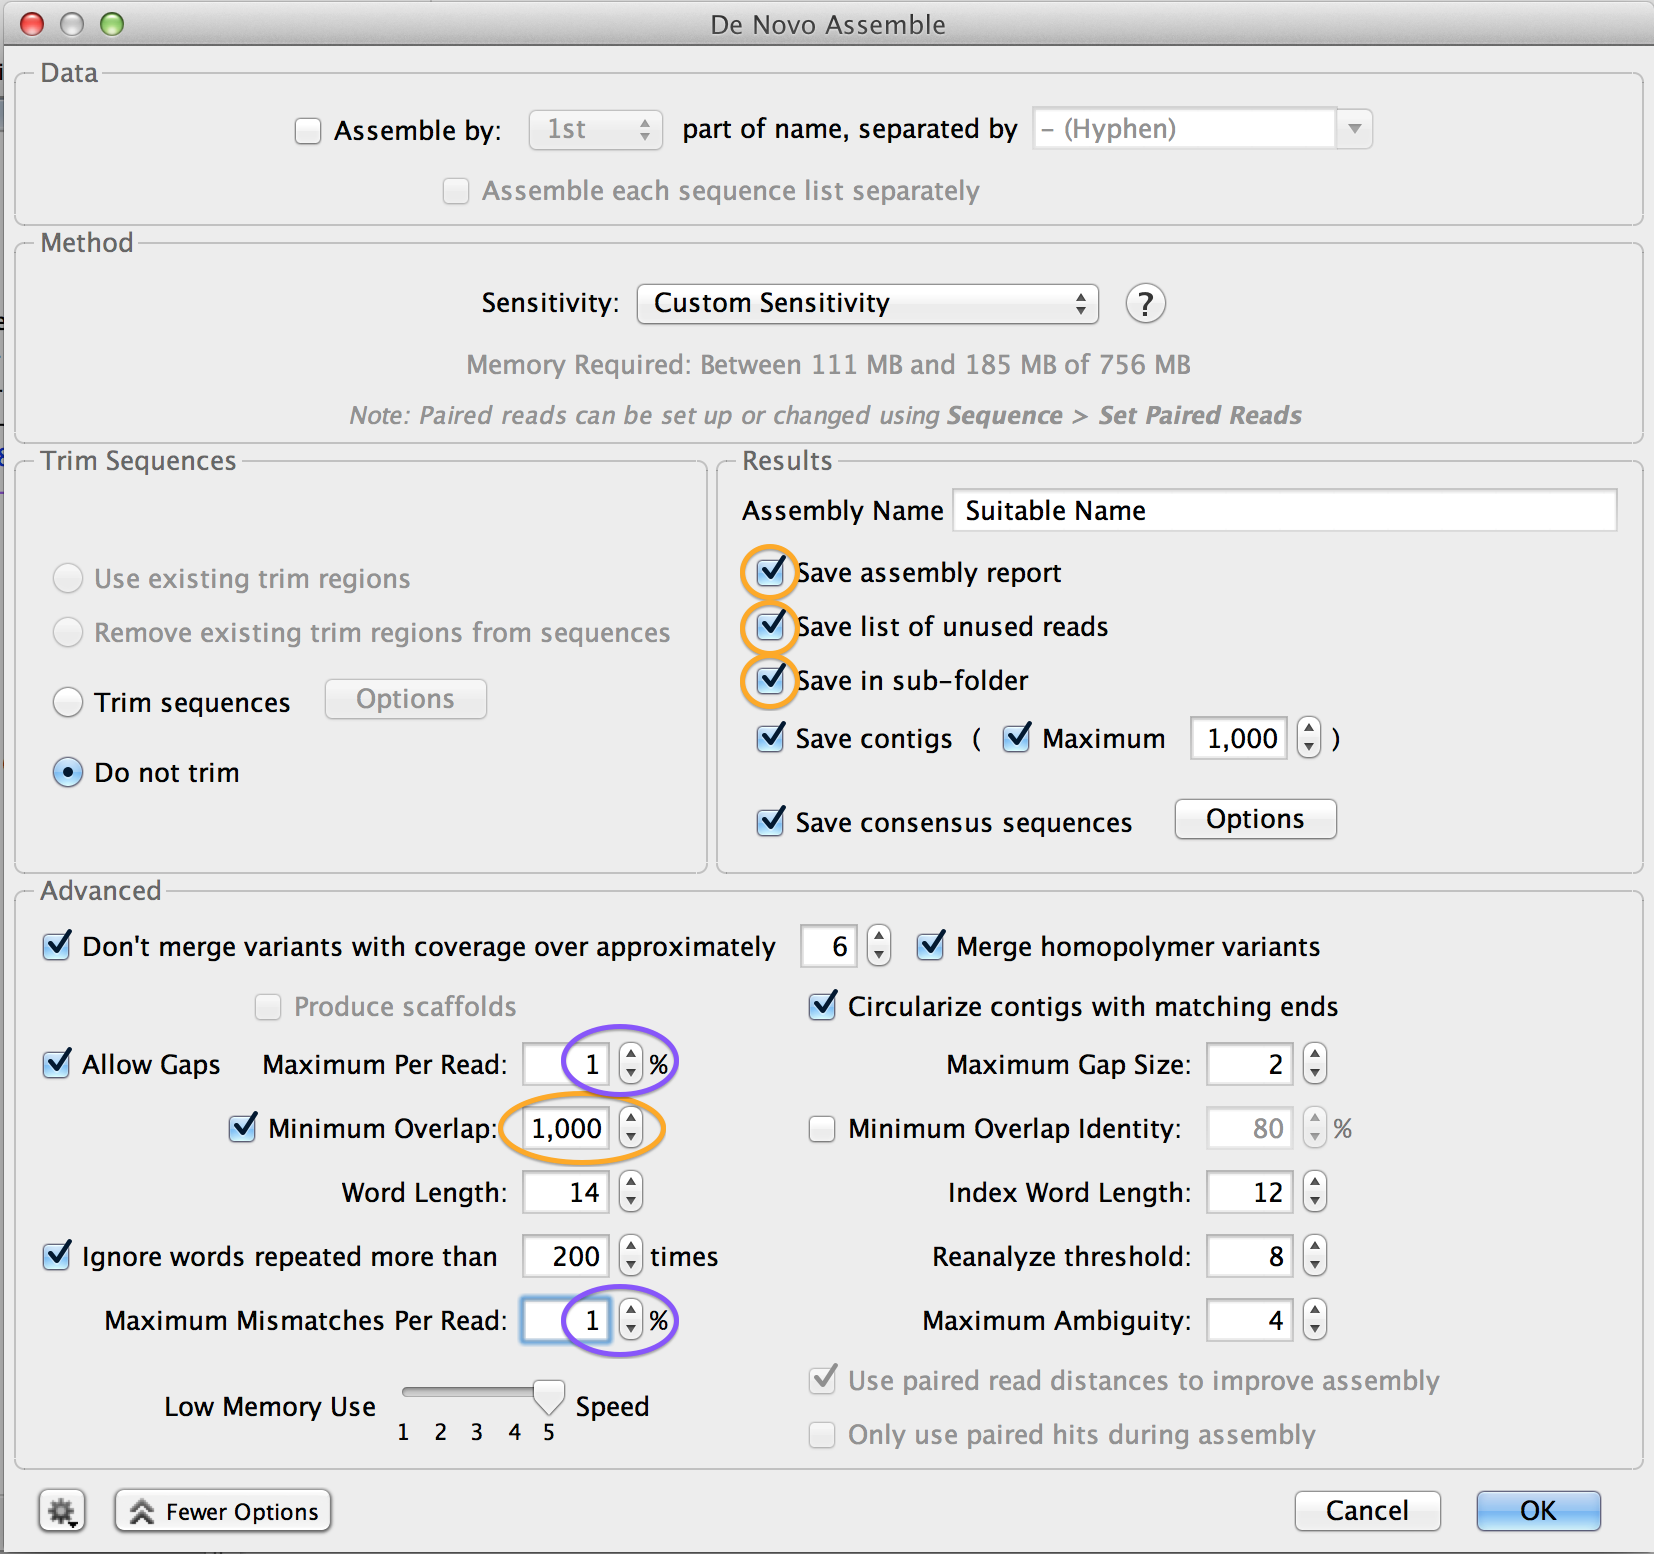
\includegraphics[width=0.5\textwidth]{assembly.png}
  \captionof{figure}{\footnotesize Assembly Popup Window}
  \label{fig:assembly}
\end{figure}

\begin{figure}[H]
  \centering
    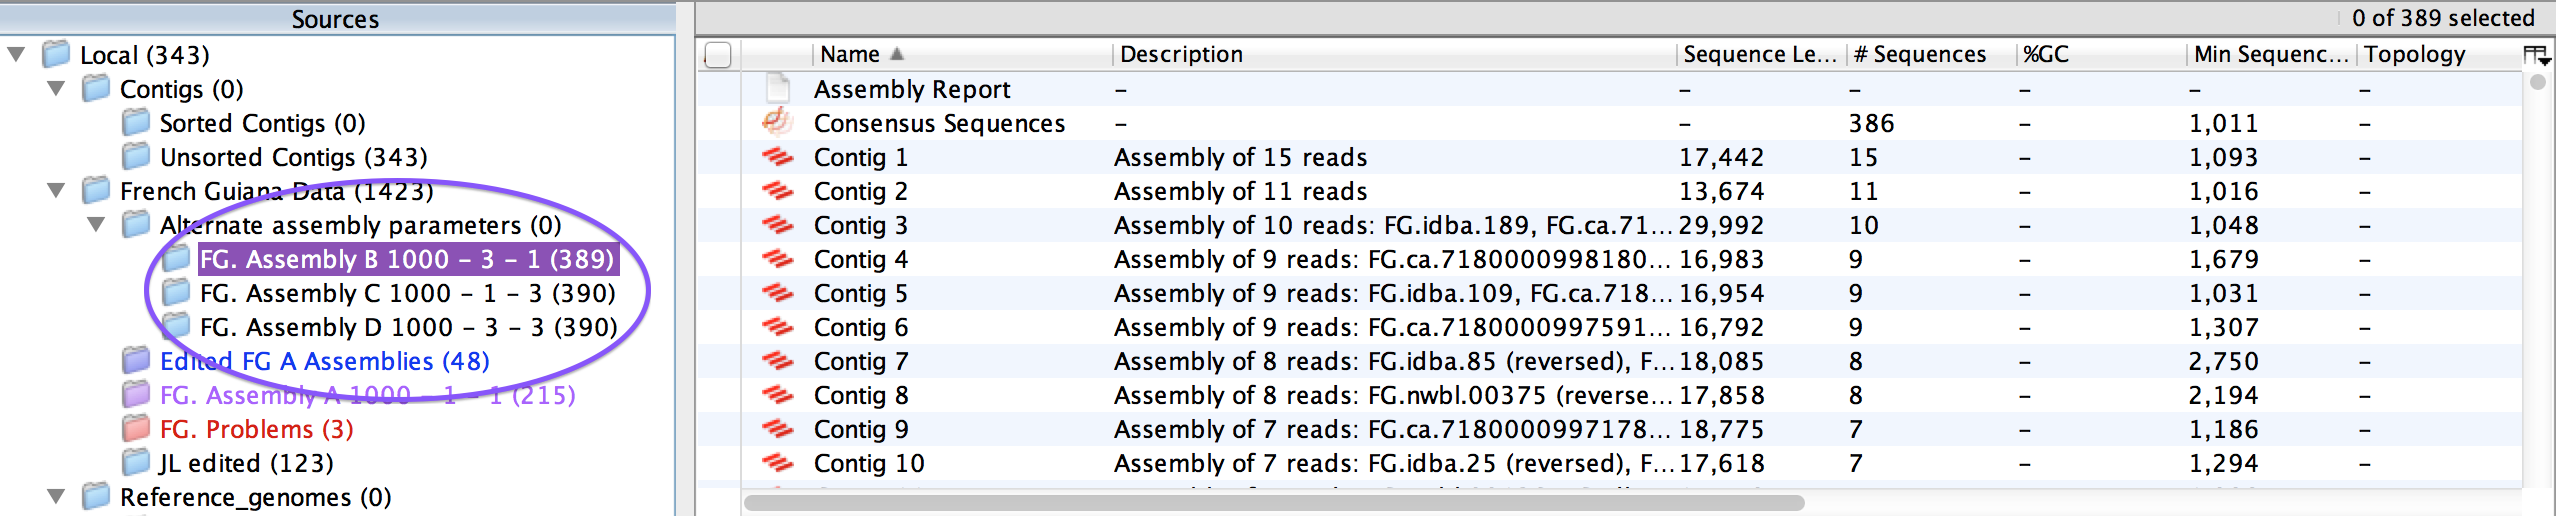
\includegraphics[width=0.7\textwidth]{assembly2.png}
  \captionof{figure}{\footnotesize Assembly Results}
  \label{fig:assembly2}
\end{figure}

For convenience, you can name your folders in the following way: `Suitable Name Minimum Overlap - Maximum Per contig - Maximum Mismatches Per contig', as seen in the purple circle in~\autoref{fig:assembly2}. In our project, we choose to use only FG. Assembly A 1000 - 1 - 1, as increasing both Maximum Per contig and Maximum Mismatches Per contig only gave us one extra supercontig.  

\newpage
\section{Blasting against Barcodes}
\label{sec:Blasting}
Barcodes are COX1 and CYTB gene sequences from individual samples. The contigs obtained are from a pool of all these samples. Using the barcodes, we can find out which contigs belong to which sample.
\\
\\
In Geneious, go to Tools, Sequence Search... Click on Add/Remove Databases, Add Sequence Database... Select Custom BLAST, give it an appropriate name and select Create from file on disk. Browse and select the file with your barcode sequences. Leave Type as Nucleotide and click OK. 
\\
\\
Before barcoding, find contigs that are unable to assemble but are longer than 8,000 bps. These may be unique mitochondrial genomes on their own. You can find these in the file called Unused contigs. Left click on their name and select Extract Regions... to give you the file in the blue circle~(\autoref{fig:extractregion}).  

\begin{figure}[H]
  \centering
    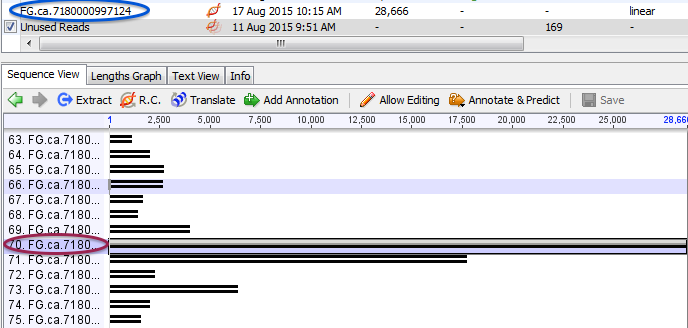
\includegraphics[width=0.8\textwidth]{extractregion.png}
  \captionof{figure}{\footnotesize Extracting unused contigs.}
  \label{fig:extractregion}
\end{figure}

For contigs that are longer than or approximately equal to 34000 bps, extract half of the sequence by highlighting the sequence and left click to select Extract Regions. Delete this region from the original sequence. Select the extracted sequence and the halved original sequence and go to Tools, Align, Pairwise alignment. This enables us to see if the two halves are from the same mitochondrion or if it is a concatenation of two mitochondria of two different species. As seen from the result in \exautoref{fig:extractregion3}, the two halves do not belong to the same mitochondria and should be barcoded separately. Otherwise, delete one copy of the mitochondria.

\begin{figure}[H]
  \centering
    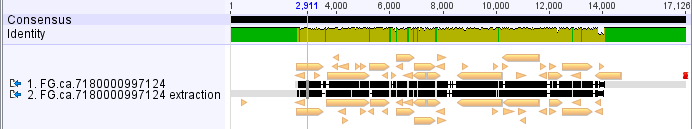
\includegraphics[width=\textwidth]{extractregion3.png}
  \captionof{figure}{\footnotesize Eliminating chimeras. Example~\ref{fig:extractregion3}}
  \label{fig:extractregion3}
\end{figure}


Select all of the supercontigs to be barcoded. Go back again to Tools, Sequence Search... Select the respective Query and under Database, you should now be able to select under Custom BLAST your newly created database. Leave other options as default and click Search~(\autoref{fig:barcoding}).

\begin{figure}[H]
  \centering
    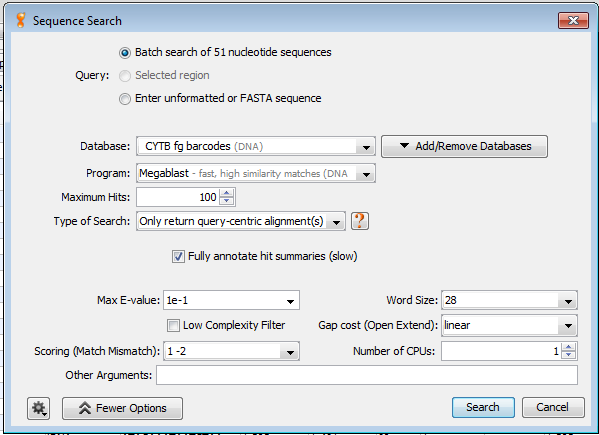
\includegraphics[width=0.6\textwidth]{barcoding.png}
  \captionof{figure}{\footnotesize Blasting against barcodes}
  \label{fig:barcoding}
\end{figure}
 
This should create new folders under Searches~(\autoref{fig:search}). Click on Columns to show \% Identical Sites and \% Pairwise Identity. Clicking on \% Identical Sites and \% Pairwise Identity will reorder the Search Hits to give you Hits with the highest similarity.You can then click on the Sequence Name of the highest similarity and return to Alignment View. This will highlight the Search Hit you have just selected in the Alignment View. 

\begin{figure}[H]
  \centering
    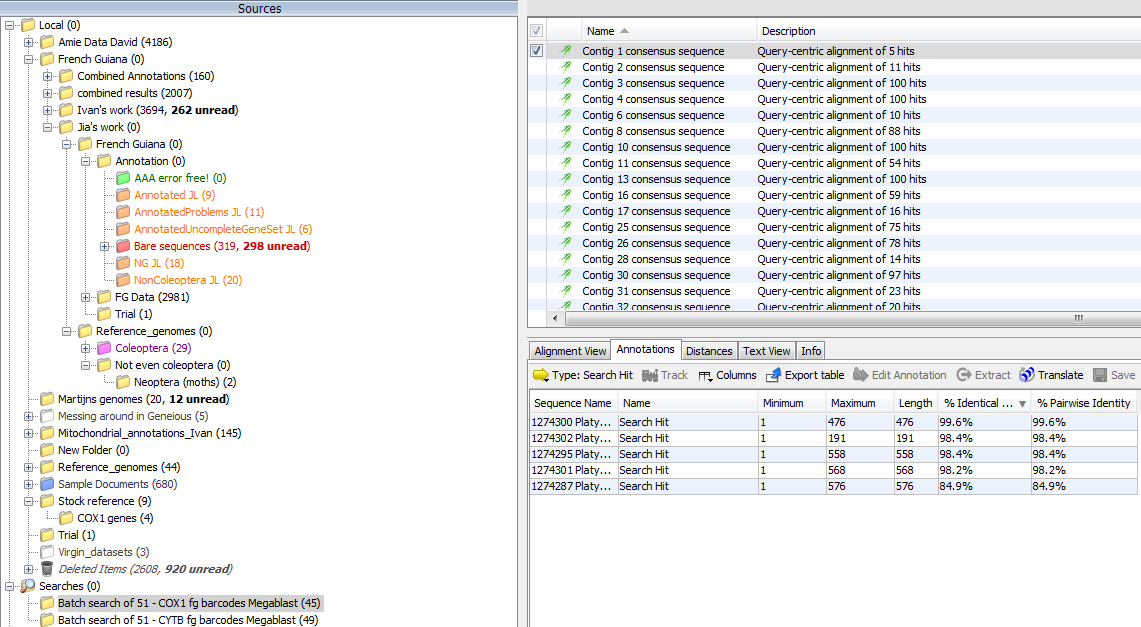
\includegraphics[width=0.8\textwidth]{search.png}
  \captionof{figure}{\footnotesize Blast search of barcodes}
  \label{fig:search}
\end{figure}

If it is a 100\% similarity, Left click the Search Hit name, Copy Name and record it down in the data sheet. At the same time return to your query folder, find the corresponding supercontig and click on the supercontig name twice, enabling you to change the supercontig name. Alternatively one can click the supercontig once and use the keyboard shortcut F2 to edit the supercontig name. Left click and select Paste to easily change the supercontig name to the title found on the barcode with the highest similarity. This is usually a string of numbers\_Name\_P1 or P2. For example, 1274645\_Staphylinidae\_P2. Some supercontigs will correspond to COX1 barcodes or CYTB barcodes of a specimen or both. supercontigs that have COX1 barcode of one specimen and CYTB barcode of another specimen are chimeras and should be removed. 

\subsection{Case Studies}
However, in the case that a Search Hit has a high \% similarity of over 99\%, record it down and note down the number of mismatches. Check through the mismatches. In some cases, it may be a M mismatch with a C. However, M represents either cytosine or adenine and hence this is not considered a mismatch, but Geneious does not see that. Also, every number should represent one species and hence there should be no more than one supercontig for each species. Mismatches may be due to editing or sequencing errors and hence Blast matches with few number of mismatches should be correct as long as each number only corresponds to one supercontig.
\\
\\
Sometimes, more than one supercontig appears to come from the same species. In \exautoref{fig:blastex}, both supercontigs gave a blast result of species number 216 for COX1. However, one gives the blast result of species number 126 for CYTB and the other 216 for CYTB. Hence, the former is a chimera which has the gene COX1 from species 216 but CYTB from species 126 and hence will be deleted. A pairwise alignment of the two sequences will give the result of \exautoref{fig:blastex}.

\begin{figure}[H]
  \centering
    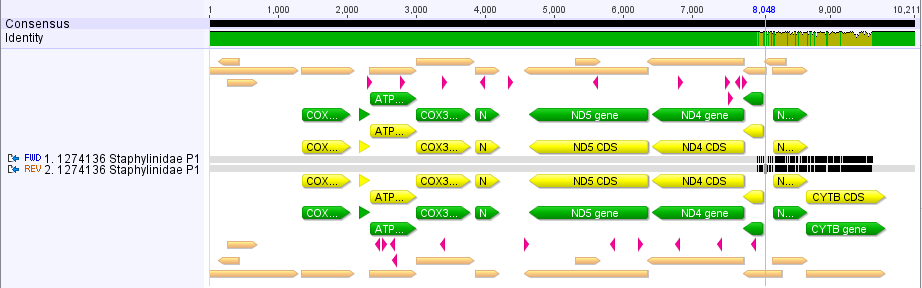
\includegraphics[width=0.8\textwidth]{blastex.png}
  \captionof{figure}{\footnotesize Pairwise alignment. Example \ref*{fig:blastex}.}
  \label{fig:blastex}
\end{figure}

\subsection{Keeping a datasheet}
Similarly, keep a record of the barcode numbers, whether they are present in CYTB and/or COX1 and which supercontigs came from which specimens, the number of mismatches it has with the Search hit and if it corresponded with both barcodes or only one~(\autoref{fig:barcodedatasheet1}). We did a second datasheet to record each supercontig's Search hit to detect chimeras~(\autoref{fig:barcodedatasheet2}).

\begin{figure}[H]
\makebox[\textwidth]{%
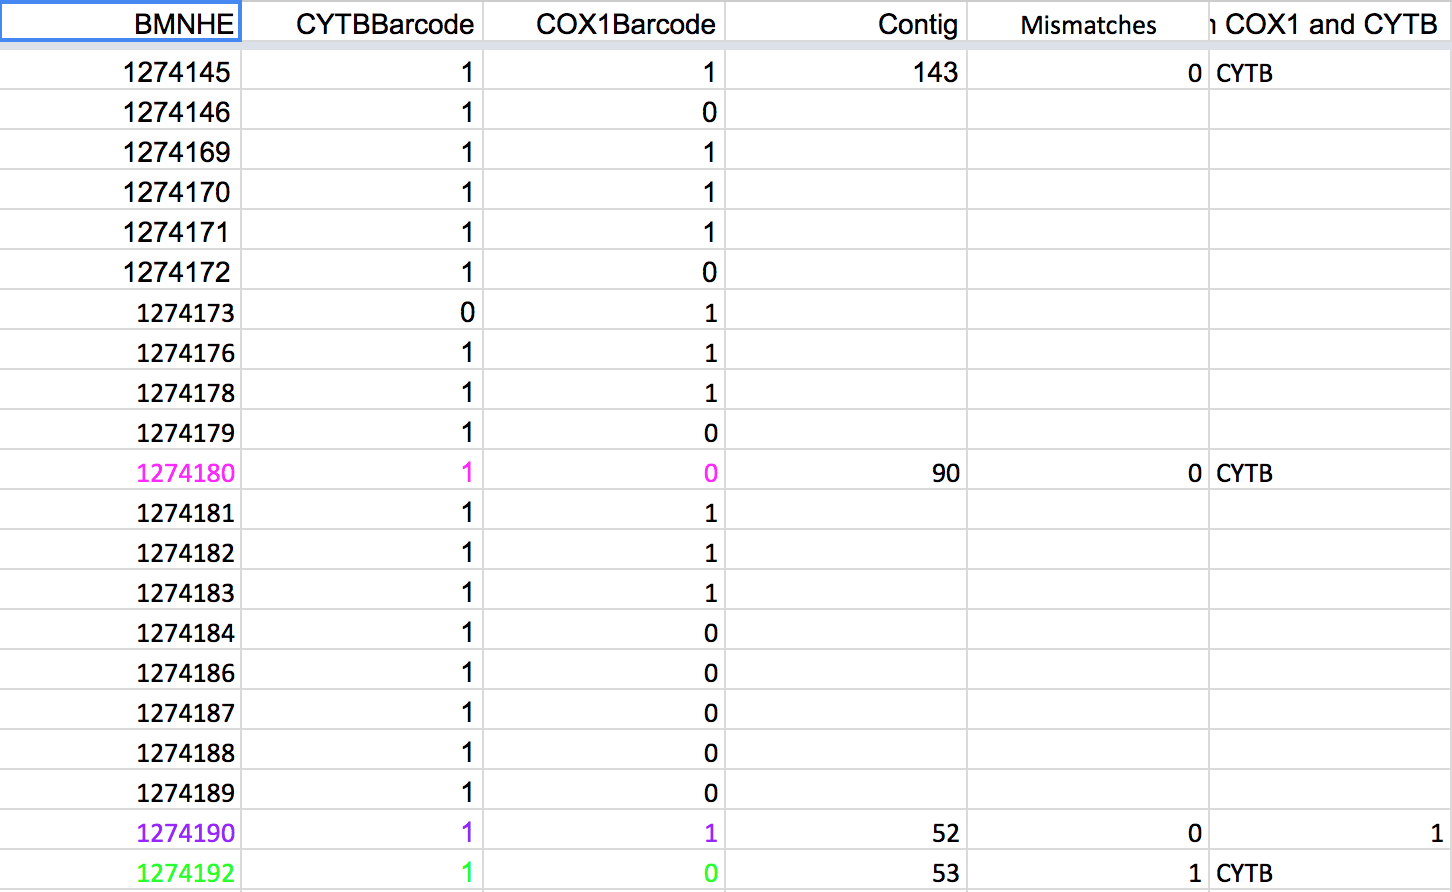
\includegraphics[width=0.5\textwidth]{barcodedatasheet1.png}%
\hfil
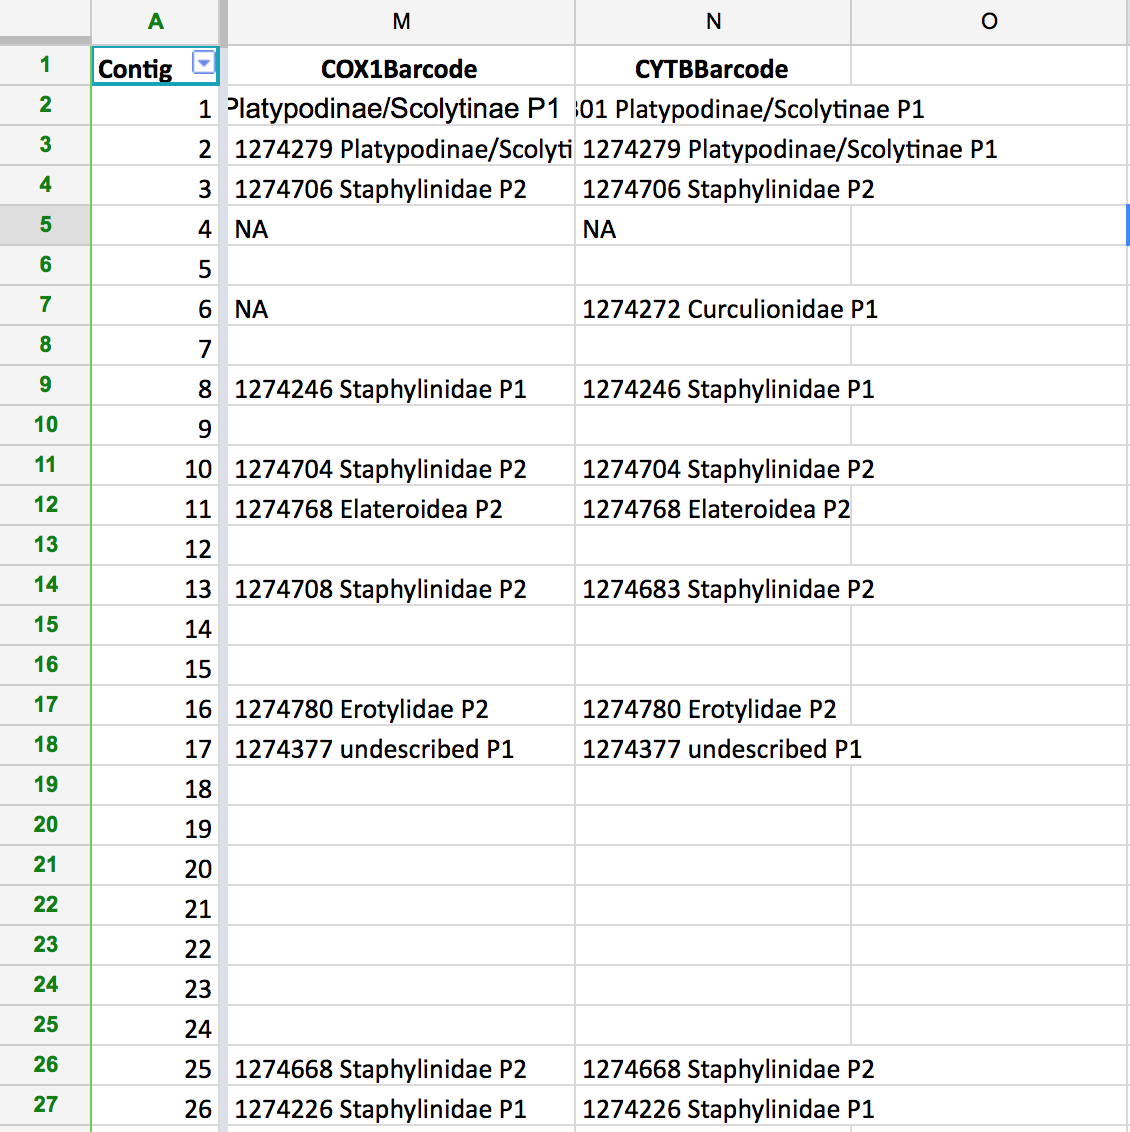
\includegraphics[width=0.3\textwidth]{barcodedatasheet2.png}%
}%\\[0.5cm] If you want some vertical space
  \captionof{figure}{\footnotesize Recording barcodes}
   \label{fig:barcodedatasheet1}\label{fig:barcodedatasheet2}
\end{figure}

\newpage
\section{Editing supercontigs}
\label{sec:Editing}
Edit the supercontigs that are barcoded. These are the supercontigs that you are interested in. 
\\
\\
Click on one of the supercontigs to see the supercontig sequence. At the right side menu, click on the orange arrow with a question mark and you can select or deselect Find ORFs. It is advised to increase the Minimum size to 200 and to change the Genetic code to the appropriate study organism i.e. Invertebrate Mitochondrial (Transl\_table 5). Selecting ORFs can help with aligning contigs that seem out of place or to increase overlapping areas of contigs. Clicking on the title of the contig selects the entire contig which allows you to thereafter click and drag the entire contig to its preferred place~(\autoref{fig:supercontig}). You can also delete the entire selected contig by pressing Delete. 
\\
\\

\begin{figure}[H]
  \centering
    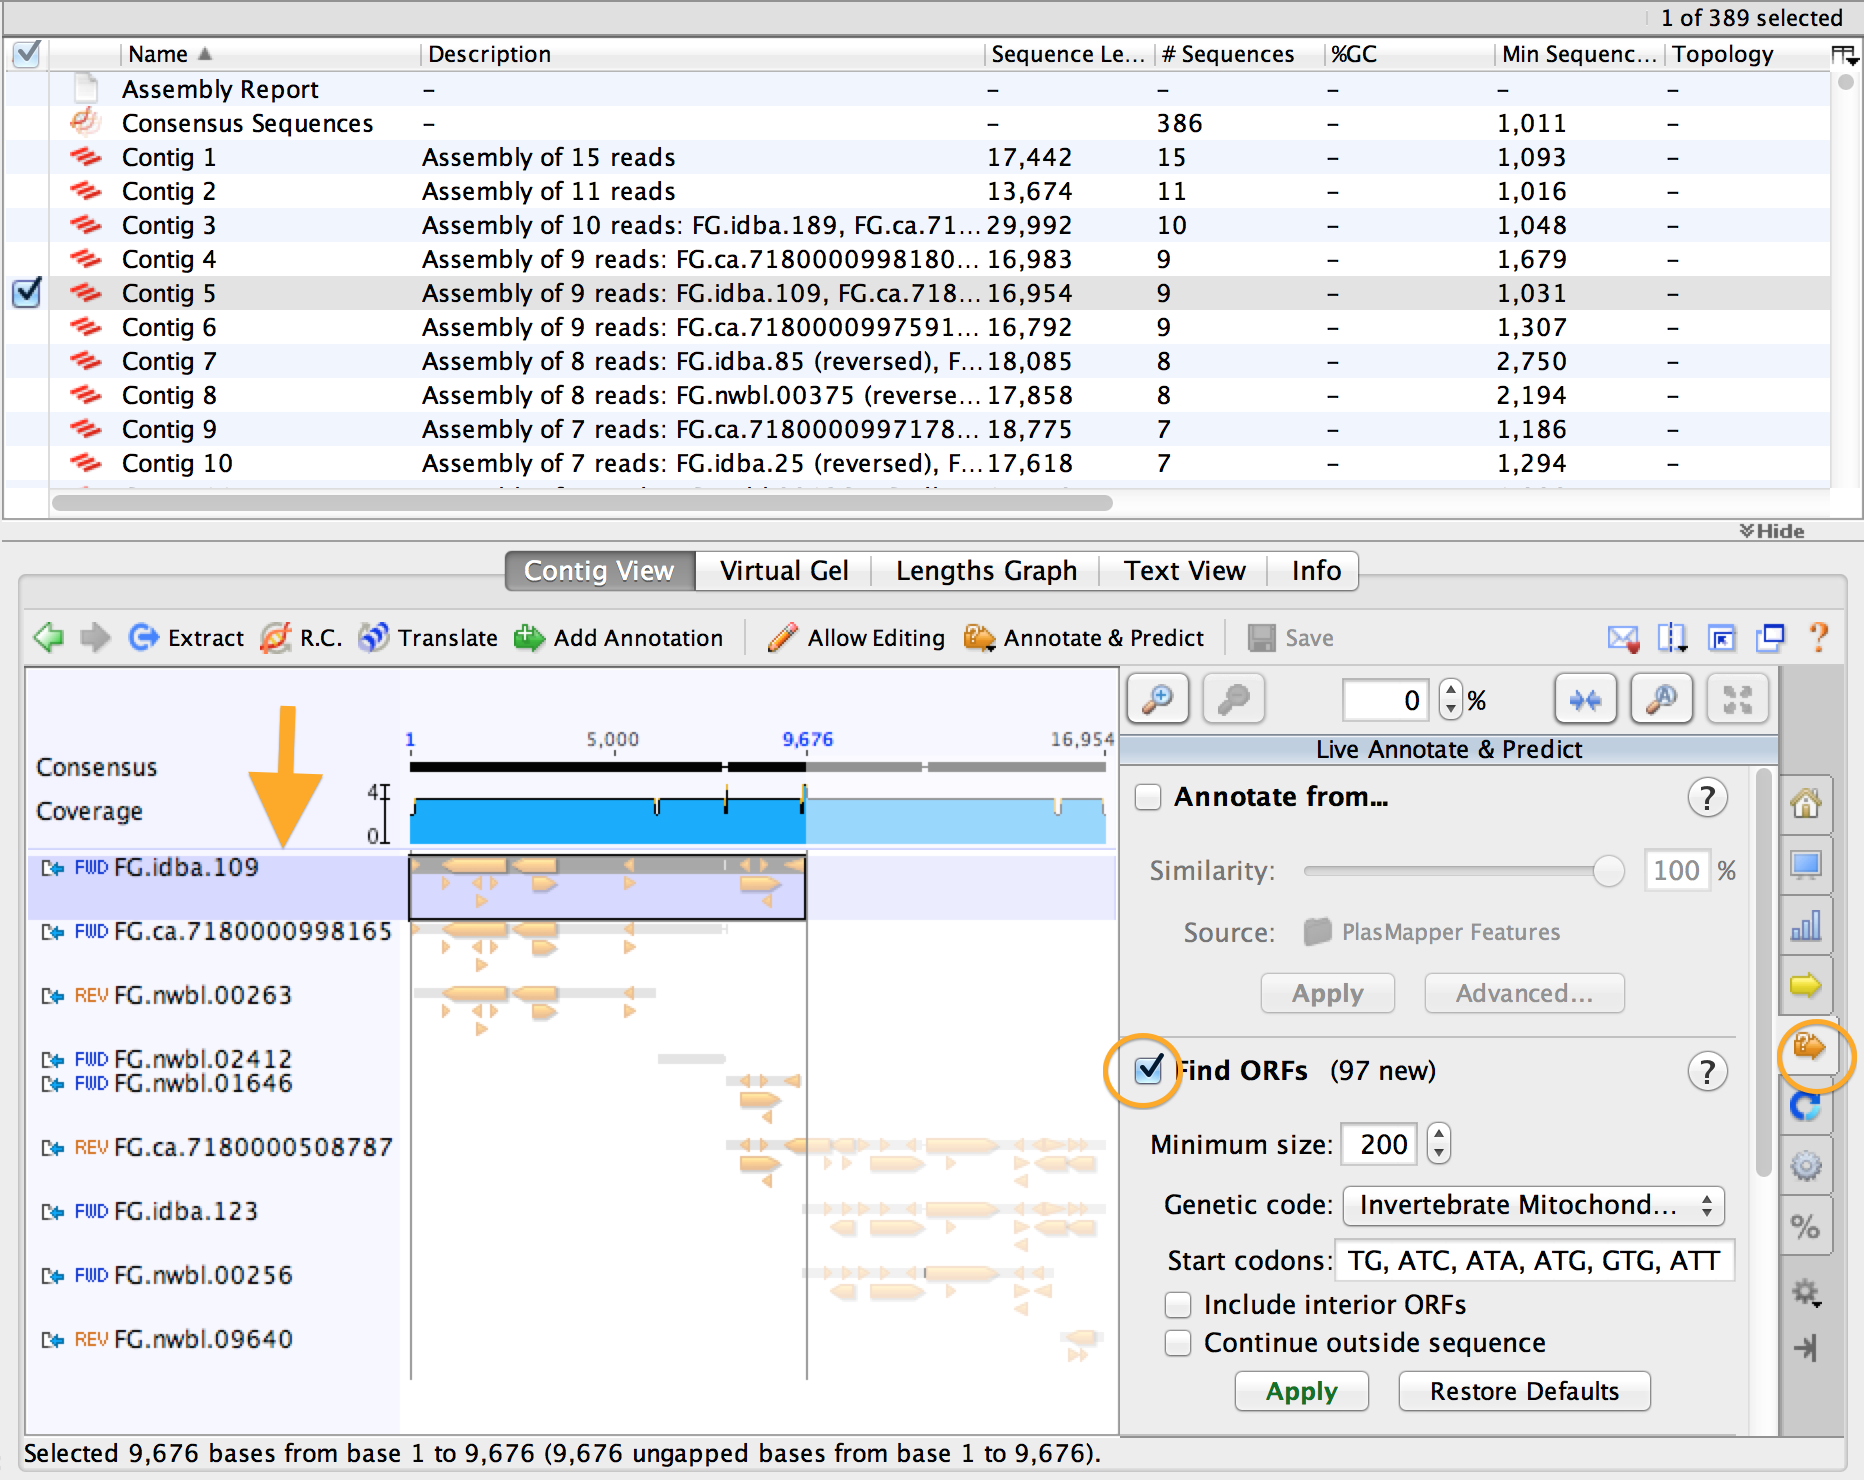
\includegraphics[width=\textwidth]{supercontig.png}
  \captionof{figure}{\footnotesize Selecting supercontigs}
  \label{fig:supercontig}
\end{figure}

After aligning the contigs, deselect Find ORFs to reveal black strips which show bases on contigs that do not agree with other contigs. Ends of contigs usually have a higher error rate and hence, ends of contigs with black strips are usually deleted~(\hyperref[fig:supercontig2]{Example \ref*{fig:supercontig2}}). To delete, highlight the sequence and press Delete/Backspace. When deleting the left end of the contig, hold Alt and press Delete/Backspace or the entire contig will shift to the left and go out of sync with other contigs. 
\\
\\
You can also add in additional bases by typing A,T,C or G. These bases will be underlined green. You can also delete bases and gaps by Delete/Backspace. Deleted bases will be underlined red. 
\\
\\
One can check for overlapping areas of contigs by highlighting sequences and pressing Ctrl-C (Copy), Ctrl-F (Find) and Ctrl-V (Paste) to paste the sequence into the search box and click Find Next. To circularise consensus sequence of supercontigs when they have overlapping ends, you have to manually edit the sequence and delete the overlapping area. Take note that you can only circularise consensus sequences but it is easier to edit and find overlapping areas using supercontigs as you can make a better informed decision of what to delete when viewing the contig errors~\secref{subsubsec:circularising}. \\
\\
To export consensus sequences, select all of the targeted supercontigs and go to File, Export, Consensus Sequence(s)... Choose 0$\%$ - Majority for Threshold, and tick Ignore Gaps. Leave other options as default and click OK. 

\subsection{Case Studies}
Here are some case studies of editing supercontigs. Do remember to check for overlaps of ends after editing when sequences are $\sim$15,000 bps, the usual length of invertebrate mitochondrion genome~\secref{sec:Editing}.

\subsubsection{Editing mismatches}
\label{subsubsec:editingmismatches}

In \exautoref{fig:supercontig2}, we would delete the end of the contig in the orange circle and leave the rest of supercontig. Problems in the purple circle cannot be resolved as no third sequences can confirm which is correct. Welcome to Biology, where nothing is either black or white. 

\begin{figure}[H]
  \centering
    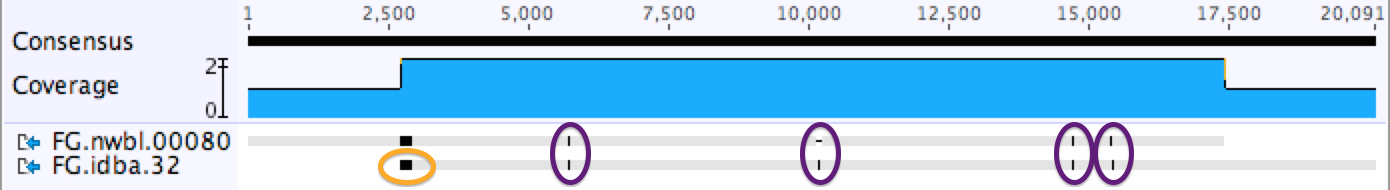
\includegraphics[width=0.9\textwidth]{supercontig2.png}
  \captionof{figure}{\footnotesize Editing supercontig Example~\ref*{fig:supercontig2}}
  \label{fig:supercontig2}
\end{figure}


In \exautoref{fig:supercontiggap}, we would ignore the gap in the purple circle as the consensus sequence will include the correct base. You can otherwise zoom in and add in the correct base manually. In the orange circle, we would delete the gap in the consensus sequence as two contigs agree that there is no nucleotide at that base position. As the sequence is much less than 15,000 bps, there is no need to find overlaps. 

\begin{figure}[H]
  \centering
    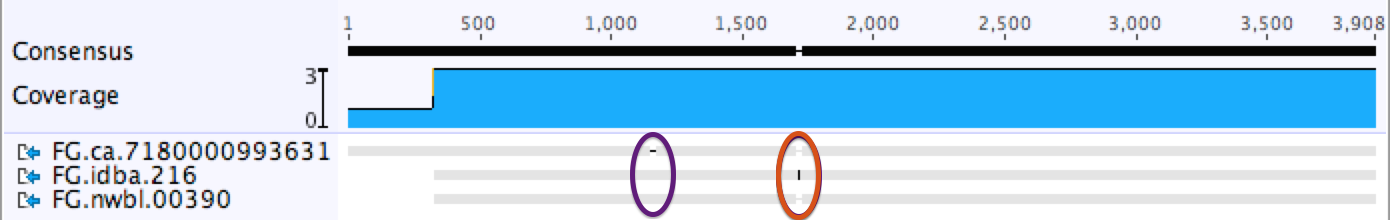
\includegraphics[width=0.9\textwidth]{supercontiggap.png}
  \captionof{figure}{\footnotesize Editing supercontig Example~\ref*{fig:supercontiggap}}
  \label{fig:supercontiggap}
\end{figure}

In \exautoref{fig:supercontigdelete}, we would delete idba.12411 as it is a short sequence that provides an error. Furthermore, there are two or more contigs that confirms the consensus sequence and hence we do not need idba.12411. We would ignore the rest of the errors as there are at least two contigs that agree with each other and thus these errors will be ignored by the consensus sequence.

\begin{figure}[H]
  \centering
    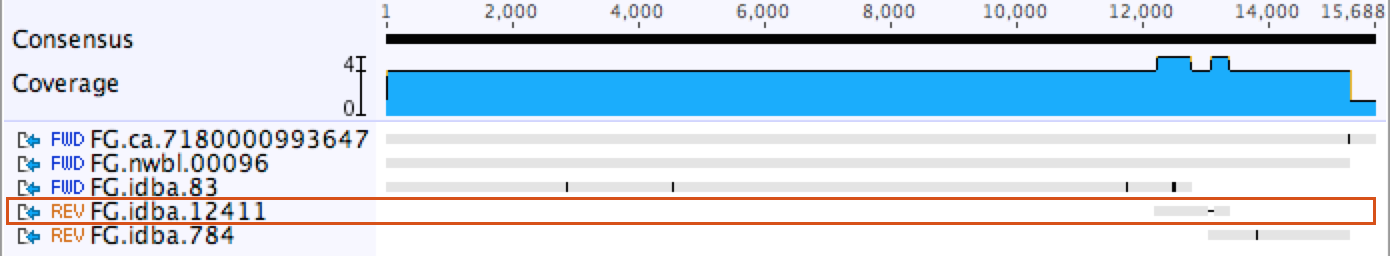
\includegraphics[width=0.9\textwidth]{supercontigdelete.png}
  \captionof{figure}{\footnotesize Editing supercontig Example~\ref*{fig:supercontigdelete}}
  \label{fig:supercontigdelete}
\end{figure}

\exautoref{fig:supercontiggd} is awesome because we do not have to edit anything \smiley~but remember to check for overlaps~\secref{sec:Editing}.

\begin{figure}[H]
  \centering
    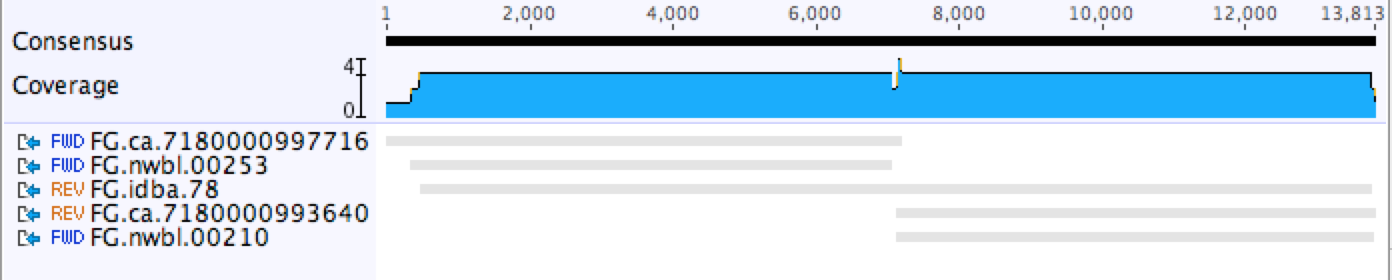
\includegraphics[width=0.9\textwidth]{supercontiggd.png}
  \captionof{figure}{\footnotesize Editing supercontig Example~\ref*{fig:supercontiggd}}
  \label{fig:supercontiggd}
\end{figure}

\exautoref{fig:supercontig4} is not awesome \frownie~but you will come across many of these. Ends in the two orange circles can be deleted. You can choose to ignore ca.7180000507897 or delete it. Zoom into the purple circles to see if the black strips of different contigs are located on the same base. If they are, they cannot be edited, record them down onto a datasheet. If they do not coincide, you can ignore them and let the consensus sequence do its job. Again, check the ends for overlaps~\secref{sec:Editing}. 

\begin{figure}[H]
  \centering
    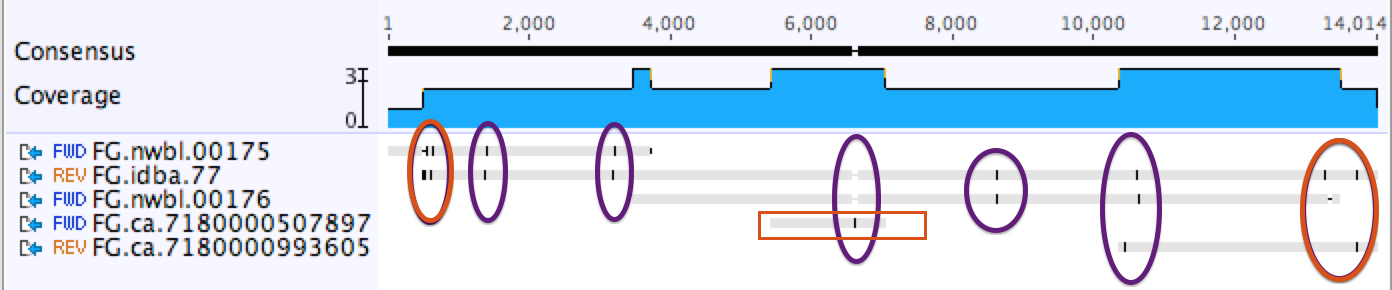
\includegraphics[width=0.9\textwidth]{supercontig4.png}
  \captionof{figure}{\footnotesize Editing supercontig Example~\ref*{fig:supercontig4}}
  \label{fig:supercontig4}
\end{figure}

In \exautoref{fig:supercontig5}, we would delete, in the orange circle, the extra base causing the gaps in two other contigs and delete the very end of nwbl.00195. The errors in the purple circles will be ignored. In the blue circle, we would delete the end of idba.91. Lastly, check for overlapping ends.

\begin{figure}[H]
  \centering
    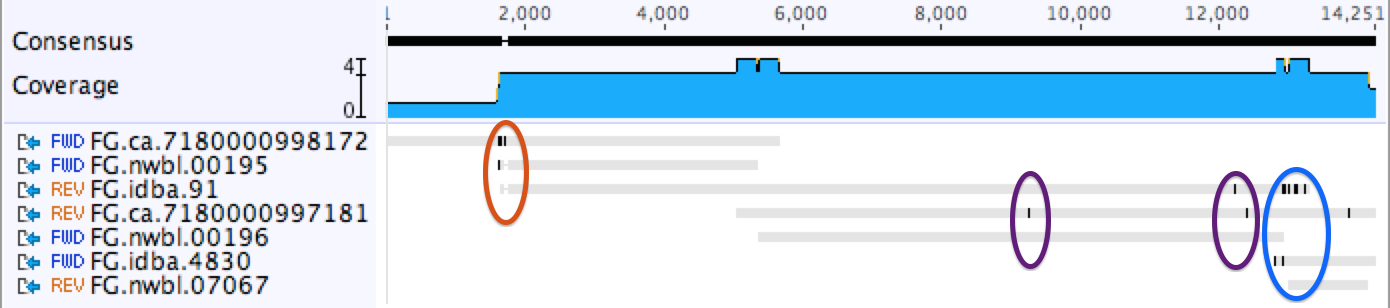
\includegraphics[width=0.9\textwidth]{supercontig5.png}
  \captionof{figure}{\footnotesize Editing supercontig Example~\ref*{fig:supercontig5}}
  \label{fig:supercontig5}
\end{figure}

\subsubsection{Editing long supercontigs}

\exautoref{fig:10A} shows how three products have been stacked to create a mammoth 36551 bp sequence. These very long supercontigs are a common problem during this process but can be easily sorted. It is advisable in these situations to ensure `Find ORFs' is ticked for this procedure as it will help to visualise the mitochondrial regions for alignment. One can also select `Find Annotations' to see what the ORF regions code for~(\exautoref{fig:10B}). Both `Find ORFs' and `Find Annotations' function is found on the `Live Annotate and Predict' Toolbar~(\autoref{fig:LAP}).
\\
\\
ORF stands for Open contiging Frames, which shows possible gene positions calculated by the program. They may not all represent real genes, but are frequently used as a guideline to find where actual genes are.

\begin{figure}[H]
  \centering
    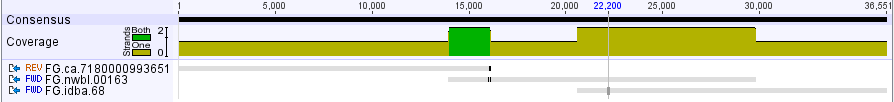
\includegraphics[width=\textwidth]{10A.png}
  \captionof{figure}{\footnotesize Dealing with long sequences Example~\ref*{fig:10A}}
  \label{fig:10A}
\end{figure}

\begin{figure}[H]
  \centering
    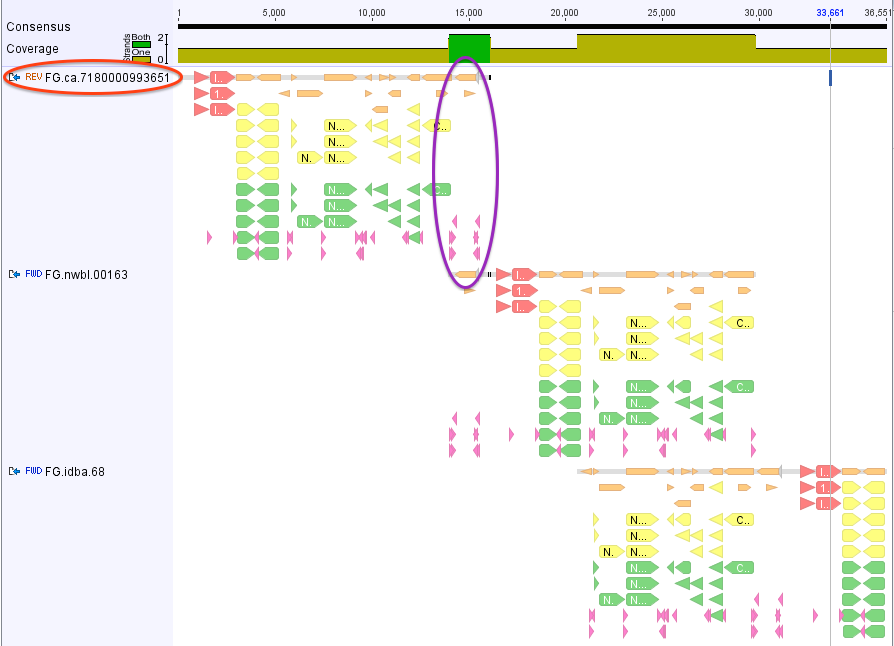
\includegraphics[width=0.75\textwidth]{10B.png}
  \captionof{figure}{\footnotesize Dealing with long sequences Example~\ref*{fig:10B}}
  \label{fig:10B}
\end{figure}

With these very large supercontigs we must confirm that the three contigs are from the same mitochondria. The overlap between nwbl.00163 and idba.68 is large, contains the same protein coding genes (as visualised by the ORFs) and is largely error free. As such we can be fairly confident that they do indeed represent the same mitochondria. However, the overlap between ca.7180000993651 is considerably smaller and might not indicate true mitochondrial identity.
\\
\\
To ensure all the contigs are from the same mitochondria it is advisable to shift them all to maximise overlap. This will increase the length over which we can look for mismatches, and thus allow us to confirm or deny mitochondrial identity. To shift a contig, ensure `Enable Editing' has been selected, click on the name of the contig on the left hand side and simply drag the contig to where you want it, relative to the other contigs. One can use the gene annotations and ORFs, as well as the zooming in function (Ctrl + Scroll) to correctly line up the contigs so that any mismatches are the result of sequence differences and not just poor alignment. In this example, ca.7180000993651 was shifted to the right to increase the overlap with nwbl.00163 and idba.68~(\exautoref{fig:10C})

\begin{figure}[H]
  \centering
    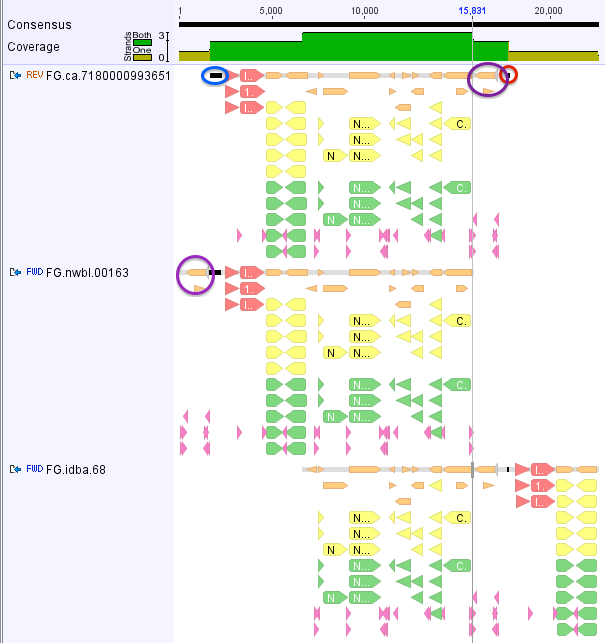
\includegraphics[width=0.6\textwidth]{10C.png}
  \captionof{figure}{\footnotesize Dealing with long sequences Example~\ref*{fig:10C}}
  \label{fig:10C}
\end{figure}

As can be seen in \exautoref{fig:10B} the sequences in the purple circle are the same, however, the sequence in the purple circle does not match that in the blue circle found in \exautoref{fig:10C}. This means that the right end of ca.7180000993651 is not the same as its left end. As sequences on both side of the many mismatches area (indicated by a black banded area) in nwbl.00163 has been confirmed by the ca.7180000993651 and idba.68, the black banded area in nwbl.00163 is likely to be correct. Hence, we will delete the two ends of ca.7180000993651 found in the purple and red circle~(\exautoref{fig:10C}).
\\
\\
Do remember to untick the `Find ORFs' and the `Find Annotations' box to see the mismatches shown as black bands that sometimes lie underneath~(\autoref{subsubsec:editingmismatches}).
\\
\\
In another more obvious example, the blue and red circle in \exautoref{fig:controlregion} do not agree with each other. After shifting nwbl.00043 to the left, we now see that the left end of idba.20 agrees with the right end of nwbl.00043 but not with the left end of ca.7180000996827. As it is two against one, we will delete the control region present in the blue circle in ca.7180000996827~(\exautoref{fig:controlregion2}). Control regions tend to be problematic, and this is one of the cases where the genes of one species has connected to the control region of another species, resulting in the chimeric ca.7180000996827.

\begin{figure}[H]
  \centering
    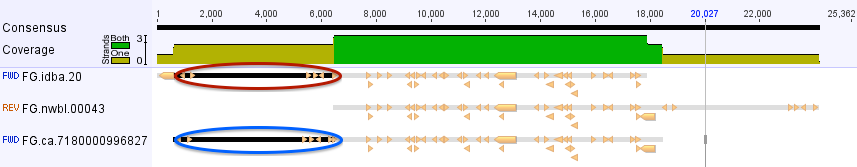
\includegraphics[width=\textwidth]{controlregion.png}
  \captionof{figure}{\footnotesize Dealing with long sequences Example~\ref*{fig:controlregion}}
  \label{fig:controlregion}
\end{figure}

\begin{figure}[H]
  \centering
    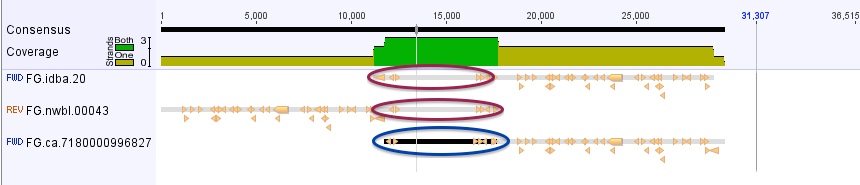
\includegraphics[width=\textwidth]{controlregion2.png}
  \captionof{figure}{\footnotesize Dealing with long sequences Example~\ref*{fig:controlregion2}}
  \label{fig:controlregion2}
\end{figure}

\subsection{Circularising sequences}\label{subsubsec:circularising}
Circularising sequences is rather tricky. There are a few ways of doing this but we recommend using Geneious.

\subsubsection{Using Python (or any other programming language). }
Likewise, to make life easier as well as to tease out more overlaps, we used the programming software Python to help us find possible overlaps. Programming softwares can find overlapping areas that we may have missed as possible overlapping areas may have only one or two errors. The search function on Geneious only returns results that have a 100$\%$ match to the search sequence. However, about 1/4 of the time, it is possible to find matches such as the one below. 
\\
\\
This particular supercontig had an overlapping area of 403 bps with only two mismatches at base positions 315 and 435. The supercontig overlaps at base positions 202-604 and 17332-17734~(\autoref{fig:overlap1}). It would not have been possible to find such a overlap using the search engine of Geneious alone. In fact, over half of our circular sequences were found using Python. Nonetheless, programming softwares are not easy to use, takes time to learn and one should not use it without knowing exactly what you are doing in case the wrong parameter was changed. They are also unforgiving on minor errors made.

\begin{figure}[H]
  \centering
    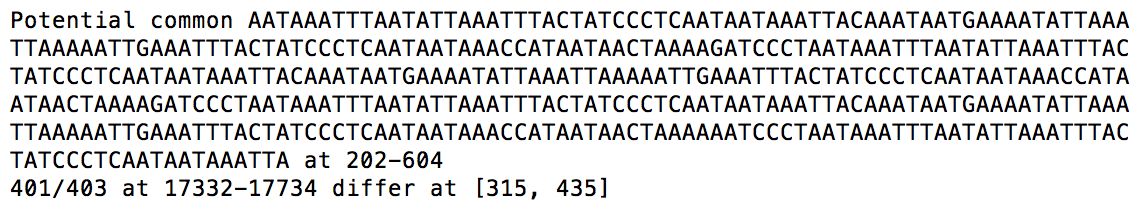
\includegraphics[width=0.65\textwidth]{overlap1.png}
  \captionof{figure}{\footnotesize Overlapping area found by Python.}
  \label{fig:overlap1}
\end{figure}

Nonetheless, for those knowledgeable in programming, this is apparently a rather easy program to code for and can be done using any programming language. When using programming softwares, start from 20 bp overlaps. If these are not found, the chance of a overlap is near null. If found, increase number of bp overlaps until it cannot be found. Then, increase the number of mismatches allowed until none can be found any further to obtain the longest possible overlap. Then, double check this sequence with Geneious and decide whether it is an overlap and thereafter delete appropriately. Overlaps should be at least 300bps long with at most 3 errors. 
\\
\\
Once overlapping areas have been found, you have to decide which overlapping area to delete. We would usually go for the area with the least contigs or with the most errors. Be very careful when deleting overlapping areas. In \exautoref{fig:overlap2a}, delete starting from the first base of the overlap sequence at 2L and till the end of the supercontig. 
\\
\\
On the other side, delete from the start of the supercontig to the first base before the overlapping sequence at 1L. If the keyboard Delete does not work, which happens at times, right-click and Delete Selected Bases. If the two sentences before seem gibberish, basically ensure that you delete only one overlapping area and not the other and not any other bases! Think before you start deleting and imagine the sequence going circular. 

\begin{figure}[H]
  \centering
    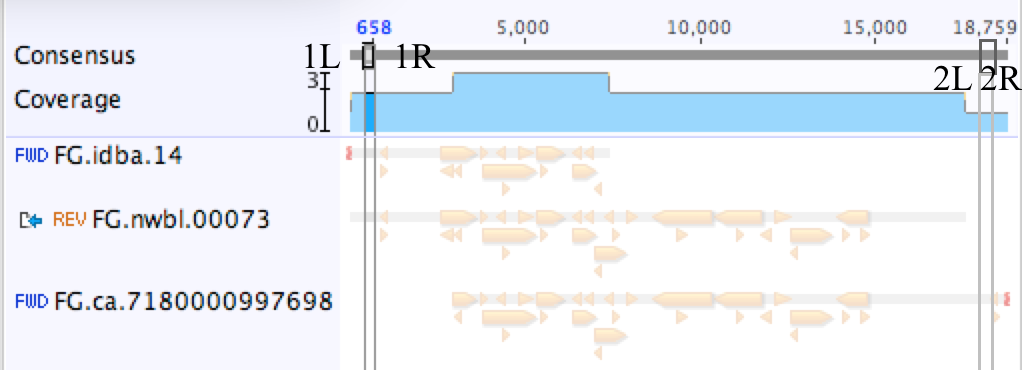
\includegraphics[width=0.8\textwidth]{overlap2a.png}
  \captionof{figure}{\footnotesize Deleting Overlaps Example~\ref*{fig:overlap2a}}
  \label{fig:overlap2a}
\end{figure}

\subsubsection{Using search function in Geneious.}
First, you can try to find overlapping areas of at least 300 bps. Check the ends of the sequences for overlap by selecting about 300 bps at either end of the consensus sequence and press Ctrl+C, Ctrl+F, Ctrl+V and click Find Next. If no overlaps are found, try checking near the ends of the supercontigs. As ends of contigs are problematic, majority of overlaps has been found here. 

\subsubsection{Making use of other information in Geneious.}
Otherwise, you can also make use of other available information. We recommend using this method to circularise sequences. Select any folder with a reference genome and Tick Annotate from... under the `Live Annotate \& Predict' Toolbar~(\autoref{fig:LAP}). This will show the rough location of all the genes~(\autoref{fig:circular1}). 
\\
\\
As we prefer to start from ND2 gene, we would delete starting from the base before tRNA-Ile at the beginning of the supercontig~(\autoref{fig:circular2}) and from tRNA-lle onwards at the end of the supercontig. This will give us a complete circular sequence with all the required genes. 

\begin{figure}[H]
  \centering
    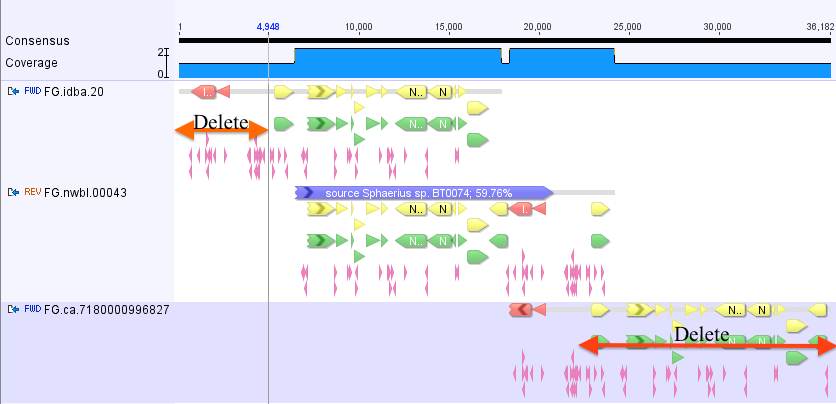
\includegraphics[width=0.7\textwidth]{circular1.png}
  \captionof{figure}{\footnotesize supercontig with annotations for reference}
  \label{fig:circular1}
\end{figure}

\begin{figure}[H]
  \centering
    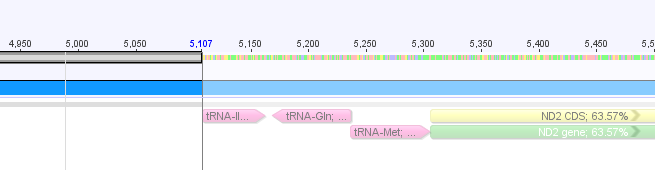
\includegraphics[width=0.8\textwidth]{circular2.png}
  \captionof{figure}{\footnotesize tRNA-Ile at beginning of supercontig}
  \label{fig:circular2}
\end{figure}
 

\subsection{Keeping a datasheet}
It is a good idea to keep a record of all the edits done on supercontigs. We recorded the initial and final number of contigs a supercontig has. We also recorded down the contigs that we deleted from each supercontig and the edits made on the supercontigs. Under edits, usual comments used were Trimmed R/L end off (contig.name) and Shifted R/L (contig.name). Number of final unresolved mismatches were recorded, if there were more than 7 mismatches, they were recorded as 100. supercontigs that have a reasonable overlap gives a 1 under able to circularise, and those unable a 0~(\autoref{fig:supercontigdatasheet}).

\begin{figure}[H]
  \centering
    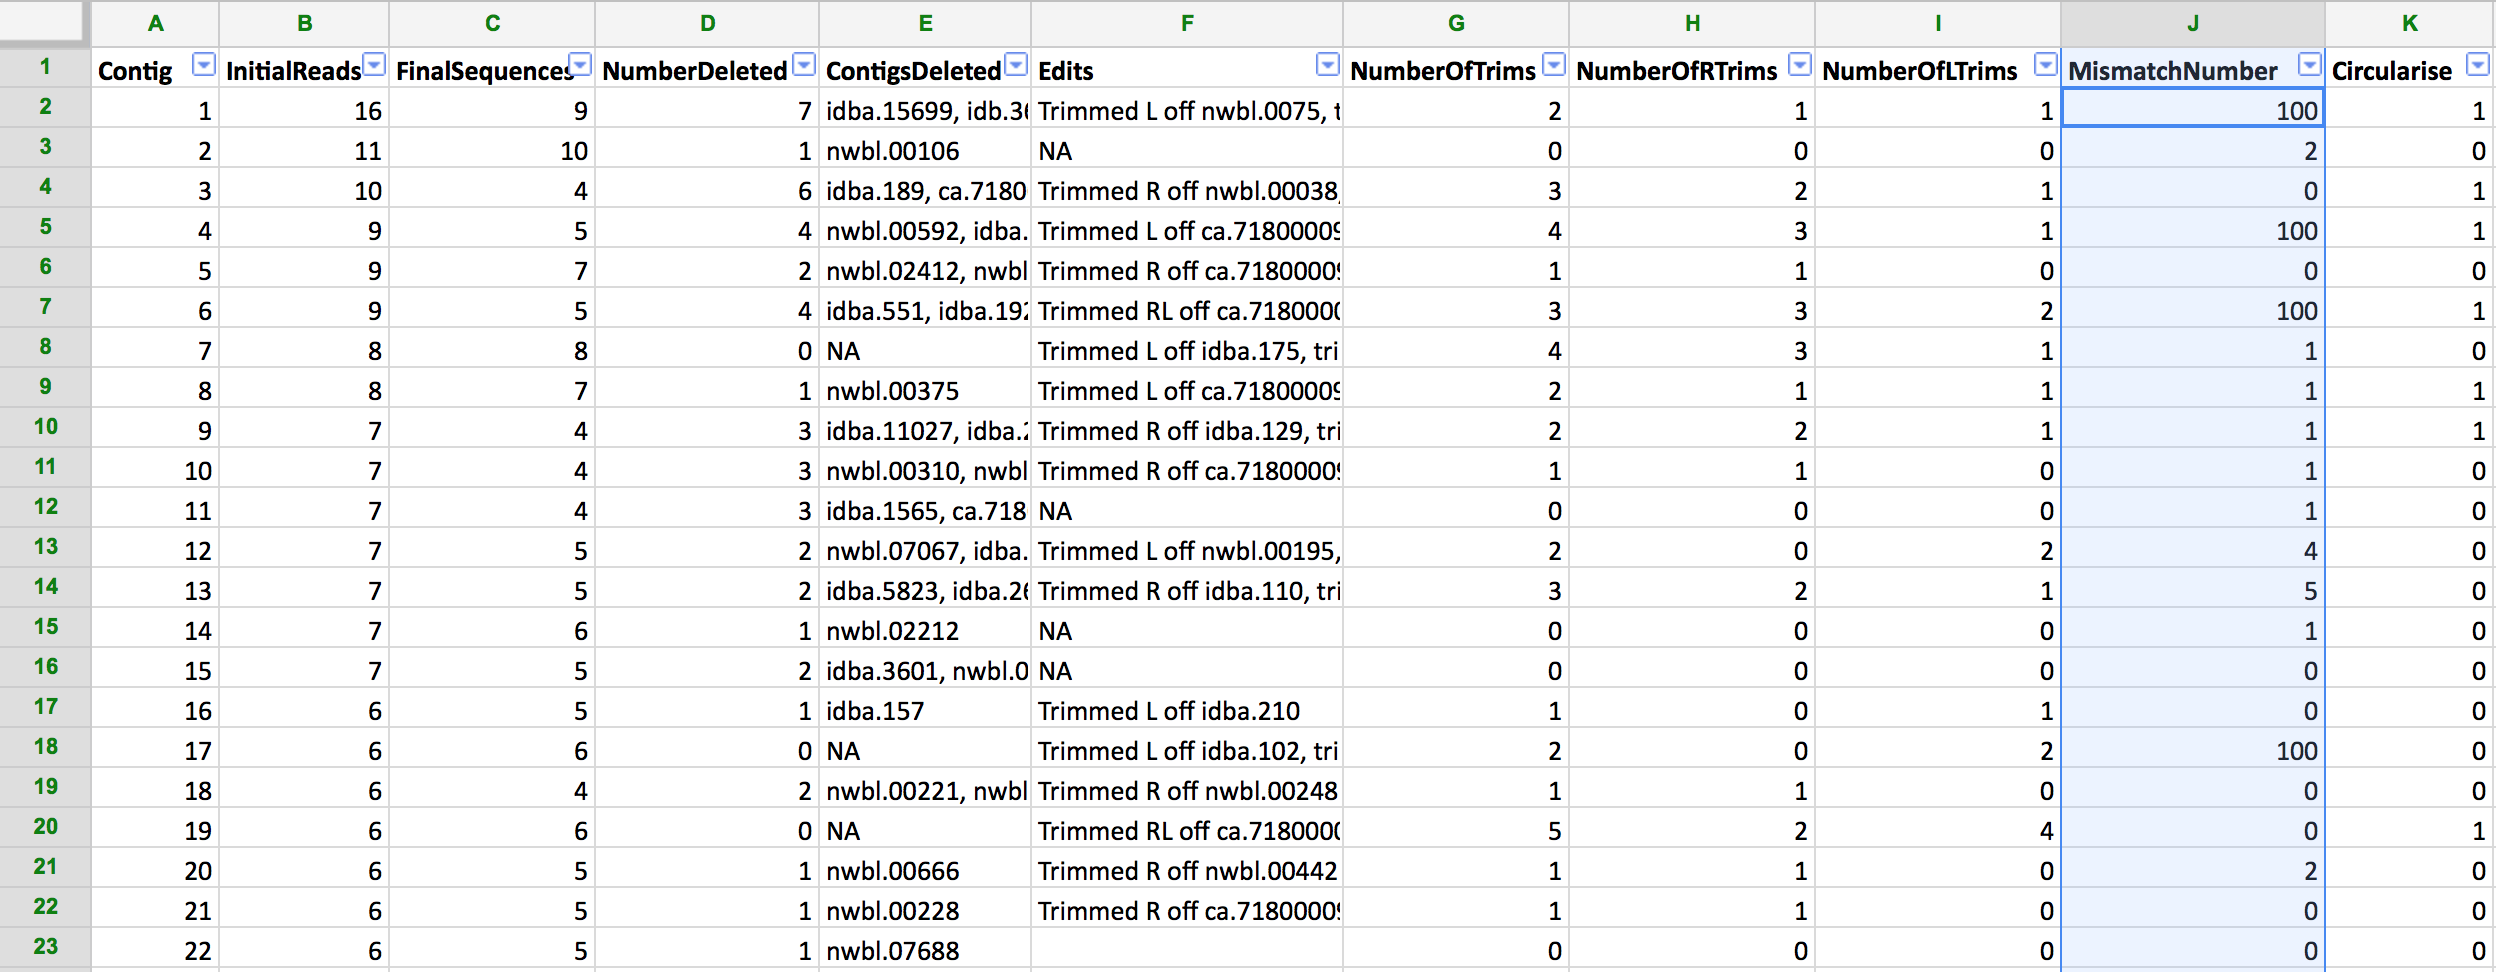
\includegraphics[width=\textwidth]{supercontigdatasheet.png}
  \captionof{figure}{\footnotesize Top headings of datasheet for supercontigs}
  \label{fig:supercontigdatasheet}
\end{figure}

\newpage
\section{Annotating genomes}
\label{sec:Annotating}
We begin the process with an un-annotated mitochondrion. Invertebrate mitochondria vary in size but are typically between 14,000 bps and 17,000 bps. Mitochondria of much lower length are likely to be just fragments whereas larger sequences could be chimeric or the result of large insertions~(\autoref{fig:annstart}). Only annotate genomes that are above 9000 bps.

\begin{figure}[H]
  \centering
    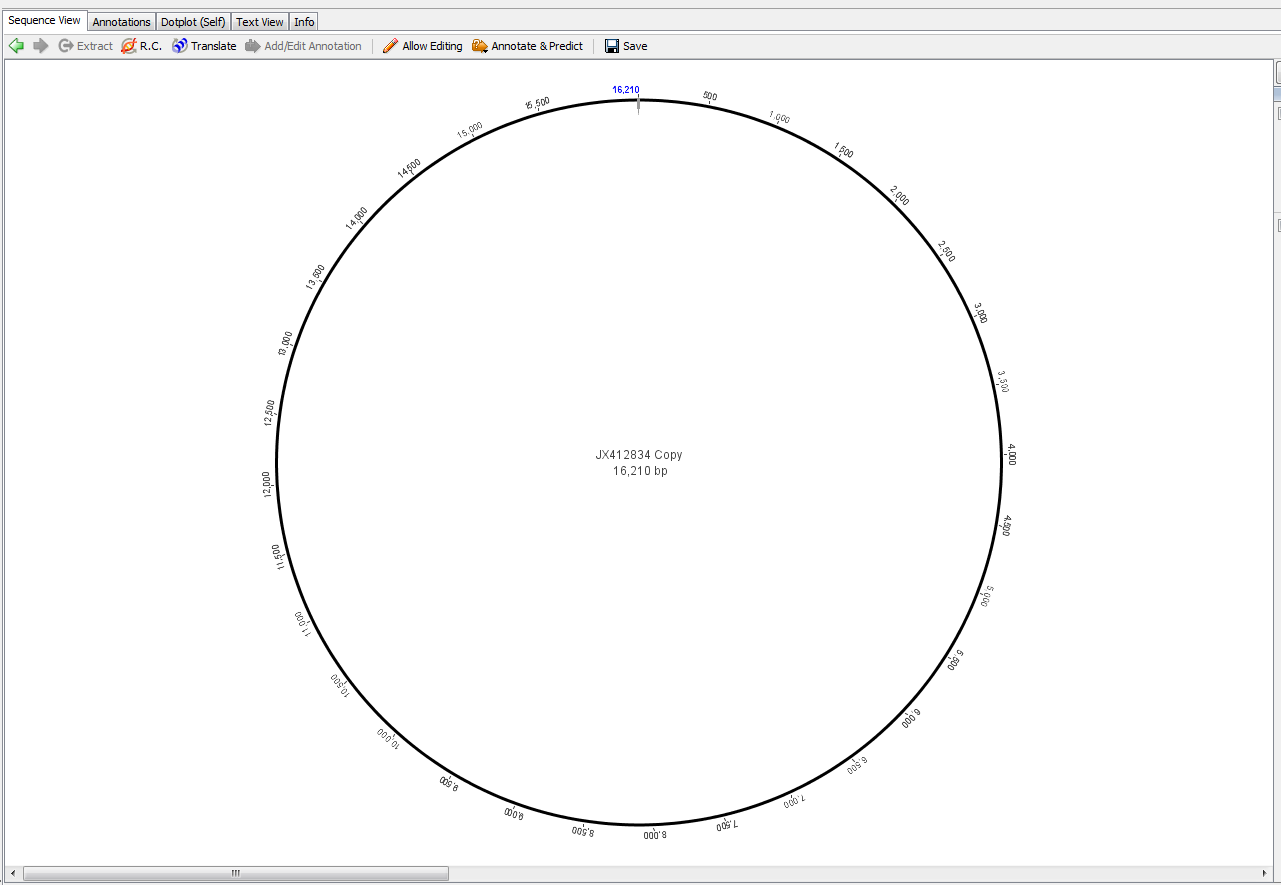
\includegraphics[width=0.6\textwidth]{annstart.png}
  \captionof{figure}{\footnotesize Un-annotated Mitochondrion}
  \label{fig:annstart}
\end{figure}

\subsection{Finding a good reference mitochondria}
Firstly we want to identify the region on the mitochondria which codes for the cytochrome c oxidase subunit 1 (COX1) as this is highly conserved. This means it is useful for determining relationships between Coleoptera taxa. 
\\
\\
Click on the `Live annotate and predict' pin~(\autoref{fig:LAP}) shown by the orange arrow to the right of the sequence in the quick tools menu. From here, it is possible to automatically look for similar sequences in mitochondria that have alcontigy been annotated and transfer them to our un-annotated trial sequence. There is a slider to determine the threshold similarity required for annotations to be shown as well as an option to select a specific folder in which to look for annotated mitochondria. The default is PlasMapper Features and should be changed to a user created folder containing a handful of well-annotated coleopteran mitochondrial genomes obtained from the NCBI database. In this case my folder is called `Stock reference'. 
\\
\\
Checking the box beside `Find Annotations' will transpose the annotations onto the un-annotated sequence. COX1 is normally the second gene/CDS cluster moving clockwise from the red rRNA-annotations. By hovering your cursor over the annotations you can see their name, length and other useful information; such as translation exceptions and any user associated notes. Clicking on one of the COX1 annotations selects the base sequence of our trial sequence over the same region. This is shown in full colour whilst everything else becomes faded. Simply copy the selected region (Ctrl + C)~(\autoref{fig:ann2}).

\begin{figure}[H]
  \centering
    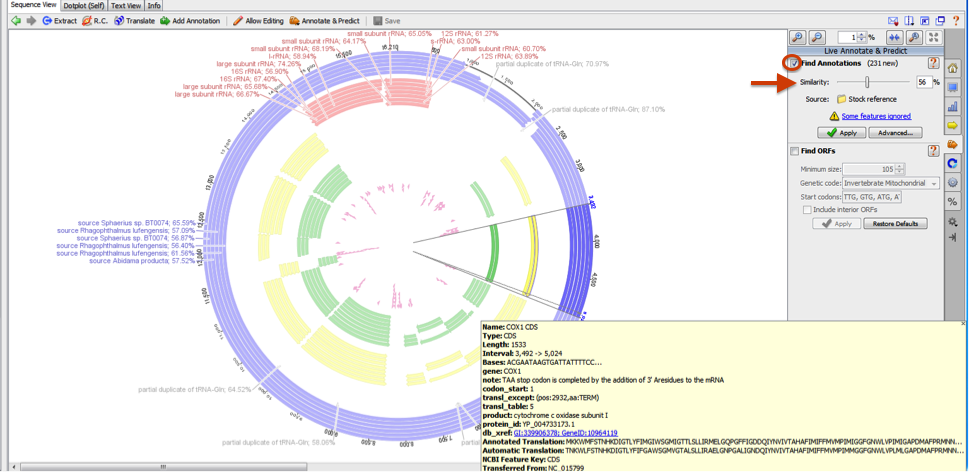
\includegraphics[width=0.8\textwidth]{ann2.png}
  \captionof{figure}{\footnotesize Selecting COX1}
  \label{fig:ann2}
\end{figure}

We shall now search this sequence within the NCBI database to find a good reference mitochondria with which to accurately transfer annotations that will require little editing afterwards. Go to the \href{http://blast.ncbi.nlm.nih.gov/Blast.cgi}{BLAST section of the NCBI website} and choose `nucleotide blast' from the given options. Paste the copied sequence (Ctrl+V) into the query box and click on the BLAST button at the bottom of the submission form~(\autoref{fig:blast}). 

\begin{figure}[H]
\makebox[\textwidth]{%
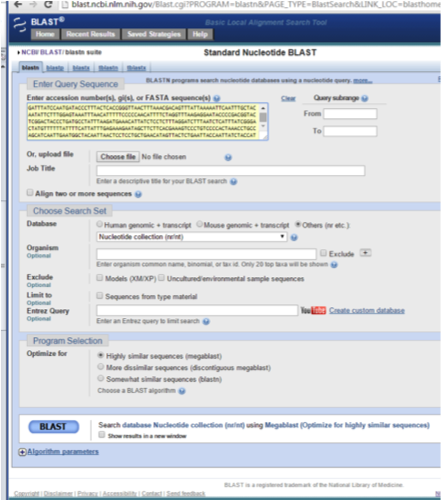
\includegraphics[width=0.48\textwidth]{blast1.png}%
\hfill    
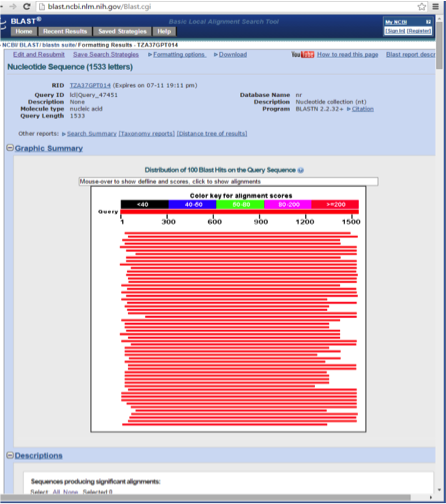
\includegraphics[width=0.48\textwidth]{blast.png}%
}%\\[0.5cm] If you want some vertical space
  \captionof{figure}{\footnotesize BLAST Search}
  \label{fig:blast}
\end{figure}

The results are presented with similar database sequences aligned to our query sequence. You can click on each of the red bars to be taken directly to them or simply scroll down the page. The hits are given in order, with those with the highest score (most similar) at the top and least at the bottom~(\autoref{fig:blast2}). Many of the hits are single gene sequences, but we are interested in complete mitochondrial genomes so annotations for other genes can also be transferred.

\begin{figure}[H]
  \centering
    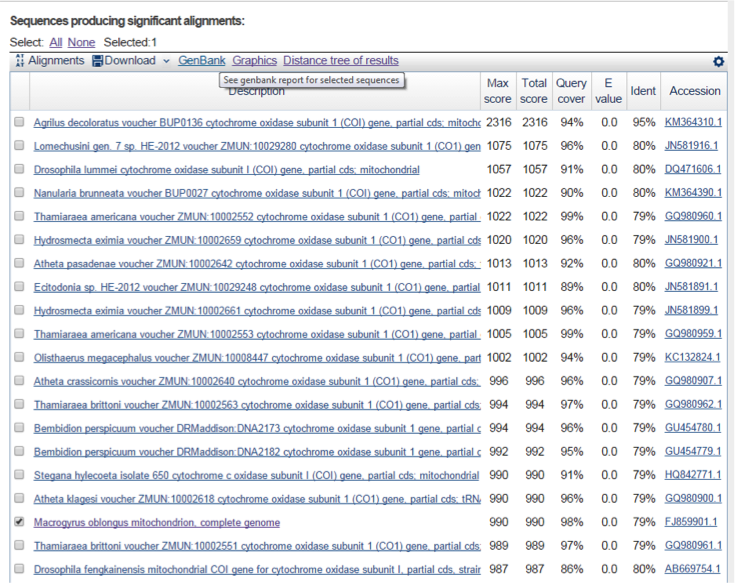
\includegraphics[width=0.8\textwidth]{blast2.png}
  \captionof{figure}{\footnotesize BLAST Results}
  \label{fig:blast2}
\end{figure}

Scroll down the list until the description is not gene specific but gives a Latin name, followed by `mitochondrion' and the tag `complete genome' i.e \textit{Macrogyrus oblongus} mitochondrion, complete genome. Select it using the checkbox and click on the link to GenBank at the top of the hit list. N.B. If there are multiple complete genomes with similar scores you can check their boxes and follow the GenBank link as normal. 
\\
\\
If there are no related complete genomes found, record the superfamily of the first hit and record the supercontig as NG. If it is not a Coleoptera, record it as NA~(\autoref{fig:annodatasheet1}).
\\
\\
The GenBank format supplies a lot of information about the sequenced mitochondrion. Importantly, note down the ACCESSION which will be used to import the annotated mitochondrial genome into Geneious later i.e. FJ859901. You can see all of the annotated features are also given here such as genes, CDS and tRNAs  - the base sequence is also given at the bottom of the page. 
\\
\\
Click on the hyperlinked organism name to be taken to the Taxonomy Browser of the NCBI~(\autoref{fig:blast3}). Here the taxonomical lineage of the species is given all the way from super-kingdom to genus. For the purposes of this lab we are interested in the super-family and family levels. Record down the superfamily name of the reference genome. Note that the latin superfamily names have the suffix -dea and the families have the suffix -dae.

\begin{figure}[H]
  \centering
    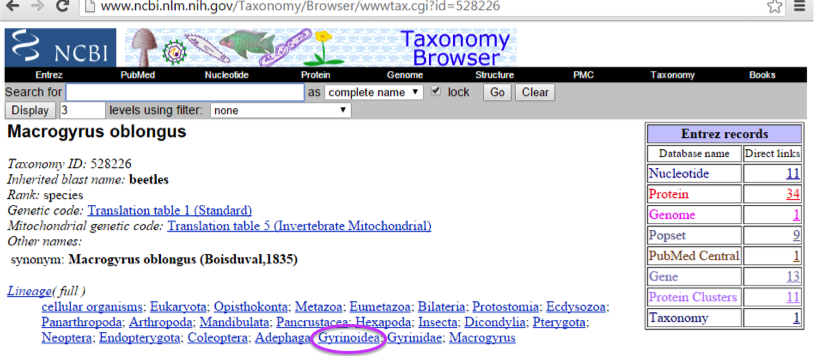
\includegraphics[width=0.8\textwidth]{blast3.png}
  \captionof{figure}{\footnotesize NCBI Taxonomy Browser}
  \label{fig:blast3}
\end{figure}

To find related species with annotated mitochondria click on one of the taxonomical rankings i.e. the super-family \textit{Gyrinoidea}, select the \textcolor{magenta}{Genome} category at the top of the page and click Go~(\autoref{fig:blast6}). All the taxa with sequenced mitochondria will then be flagged which is useful for constructing a robust database of annotated reference genomes to speed up the annotation process for un-annotated sequences later.

\begin{figure}[H]
  \centering
    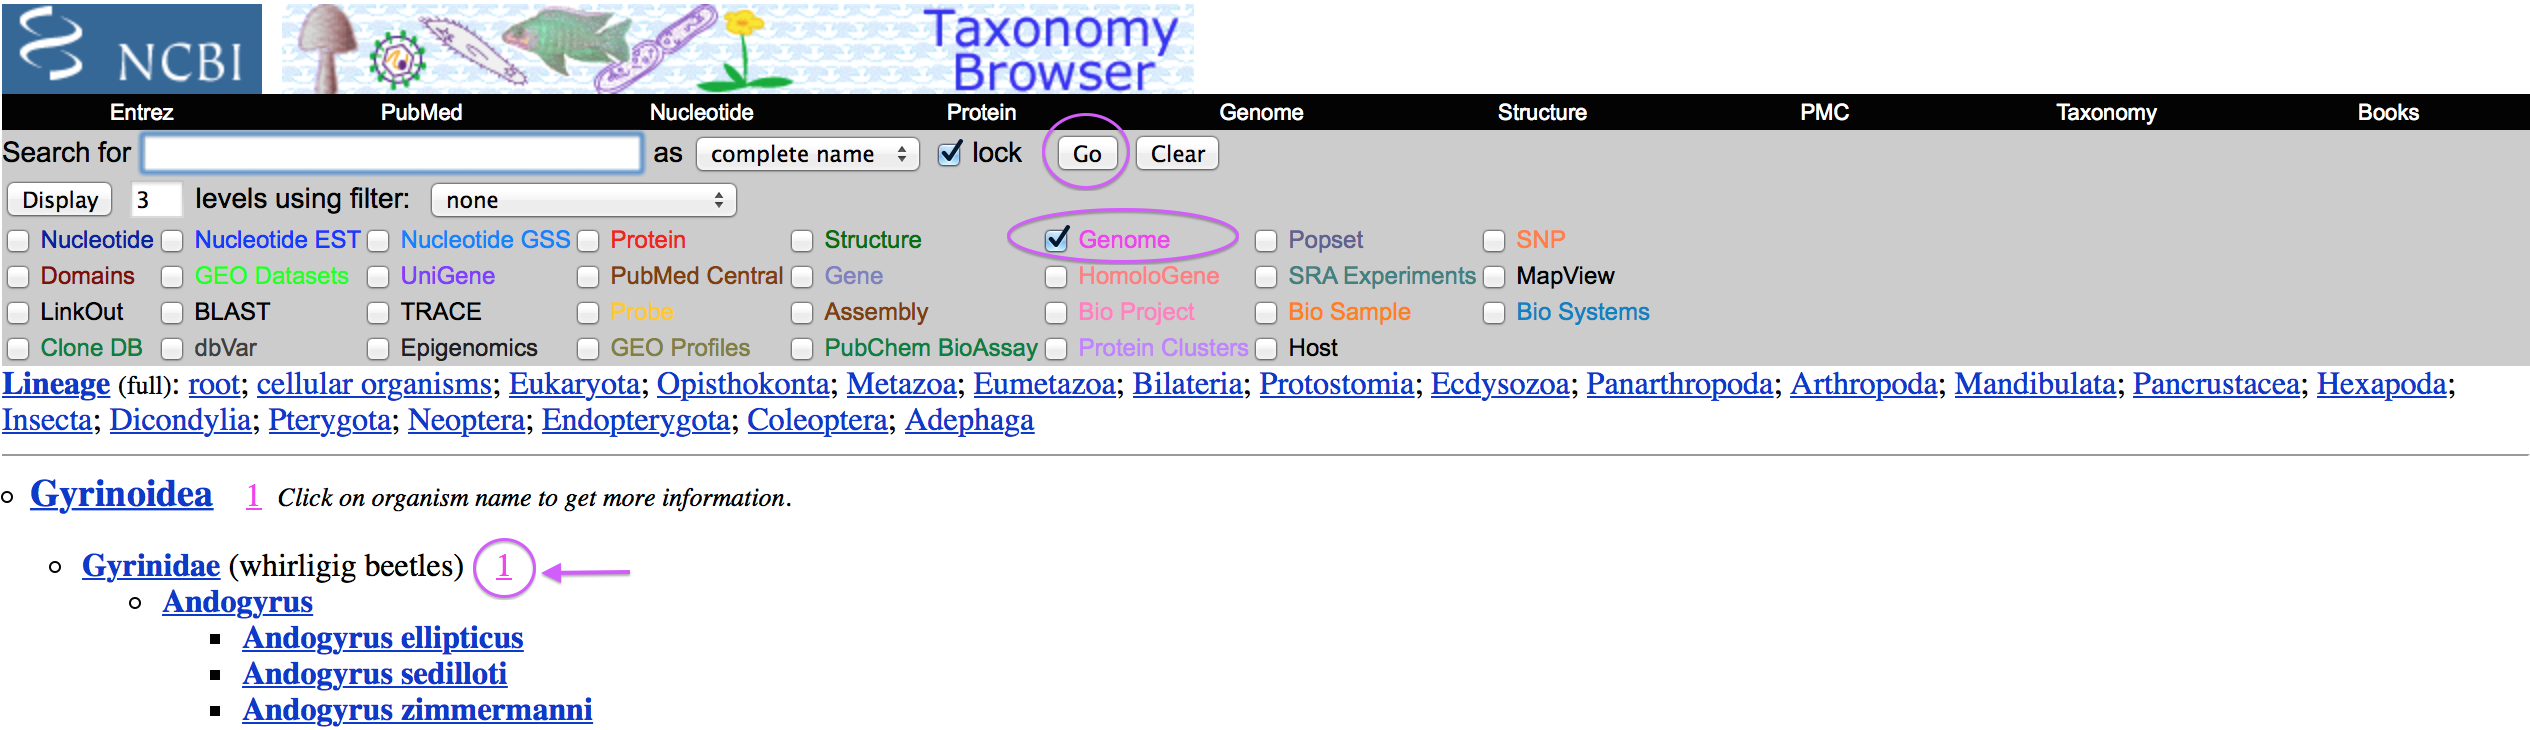
\includegraphics[width=0.8\textwidth]{blast6.png}
  \captionof{figure}{\footnotesize Fully annotated mitochondrial reference genome}
  \label{fig:blast6}
\end{figure}

Having determined the species lineage using the taxonomy browser, we can return to Geneious and import the annotated mitochondria. Select the NCBI logo in the sources pane on the lefthand side of Geneious and search using the ACCESSION key from GenBank that we acquired earlier. The fully annotated mitochondrial reference genome can now be seen~(\autoref{fig:blast4}).

\begin{figure}[H]
  \centering
    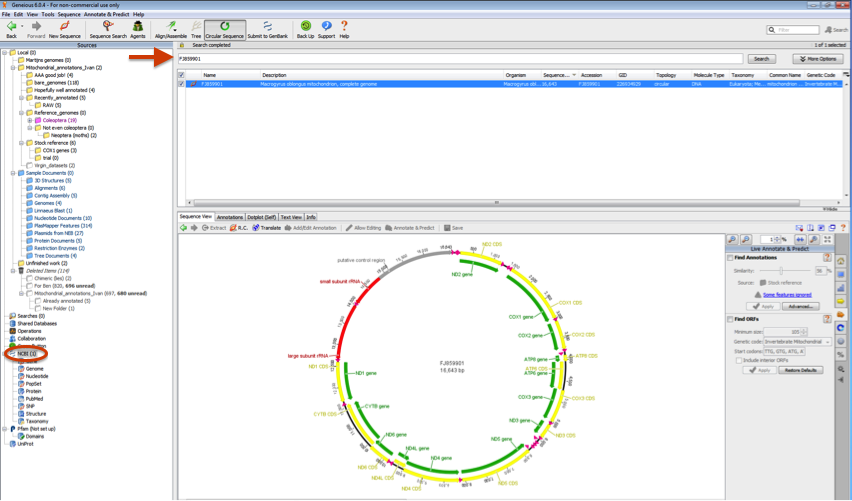
\includegraphics[width=0.6\textwidth]{blast4.png}
  \captionof{figure}{\footnotesize Fully annotated mitochondrial reference genome}
  \label{fig:blast4}
\end{figure}

%\begin{wrapfigure}{L}{0.4\textwidth} \vspace{-20pt}
  %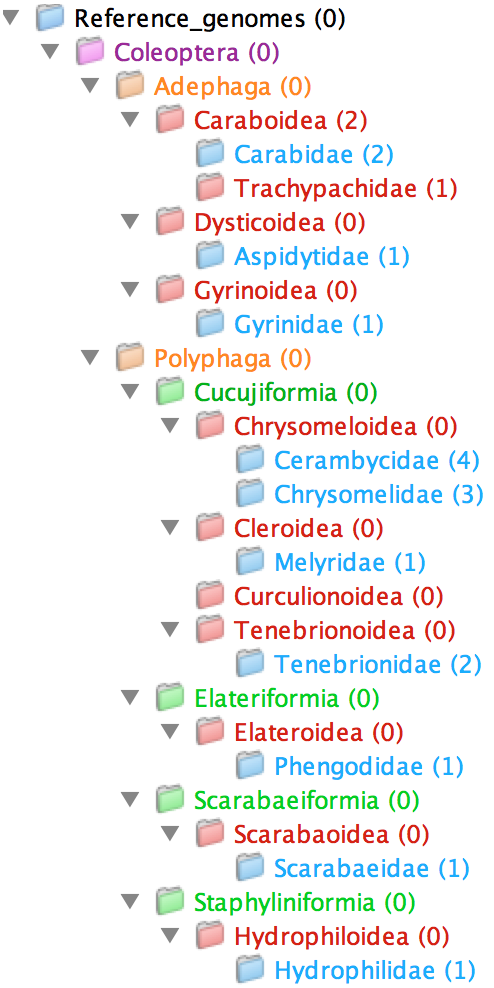
\includegraphics[width=0.32\textwidth]{blast5.png}
  %\caption{\footnotesize Folders}
  %\label{fig:blast5}
%\end{wrapfigure}

%\begin{figure}[H]
  %\centering
    %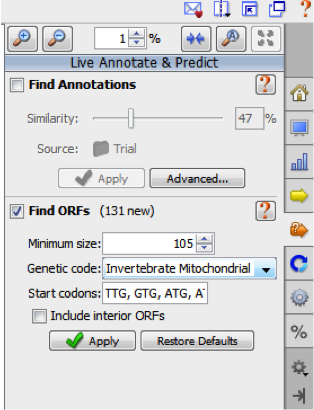
\includegraphics[width=0.3\textwidth]{LAP.png}
  %\captionof{figure}{\footnotesize `Live Annotate \& Predict' toolbar}
%  \label{fig:LAP}
%\end{figure}

\subsection{Transferring Annotations}
\label{subsec:Transferring}
Drag and drop (or alternatively copy and paste) a copy of this file to a new folder, called `Trial' here, and place another copy into the simple taxonomic reference tree you are building using information from the NCBI taxonomy browser. For example, I have placed the annotated `\textit{Macrogyrus oblongus} mitochondria' into a newly created folder to match its family classification of \textit{Gyrinidae}~(\autoref{fig:blast5}). This will enable us to find it quickly in the future if we need to re-use this reference and will ultimately provide a reference database which can be given to other scientists working on similar projects.
\\
\\
Select the original un-annotated genome that we started with and use the tools on the right to find annotations (can be quickly mapped using Ctrl+Shift+A). This time select the `Trial' folder as the source which contains only the reference mitochondrial genome found using the NCBI BLAST. Check that all 13 gene annotations are present and in the direction as seen in this example~(\autoref{fig:ideal}). If not all 13 gene annotations are present, reduce the Similarity percentage. However, when doing so, some smaller genes, such as ATP8 may appear at other places. Take note to delete these incorrect gene annotations after applying the annotations. Refer to Section~\ref{missinggene} if not all 13 gene annotations can be found. 

\begin{figure}[H]
  \centering
    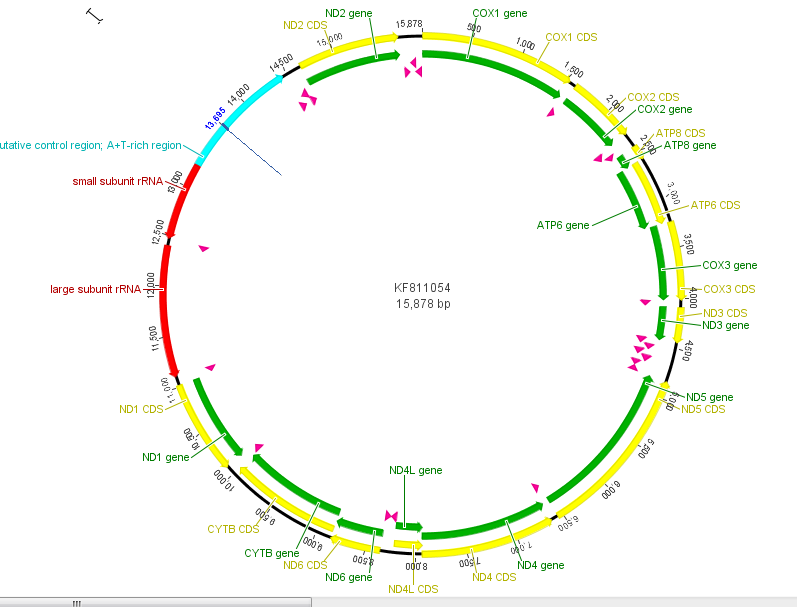
\includegraphics[width=0.7\textwidth]{ideal.png}
  \captionof{figure}{\footnotesize Example of a nicely annotated mitochondrial genome}
  \label{fig:ideal}
\end{figure}

Click the `Apply' button to transfer these annotations to the un-annotated sample mitochondrion, at which point their colours will become solid rather than faded. You can now unselect the Find Annotations tick box and the annotations will remain. 
\\
\\
On the same `Live Annotate \& Predict' toolbar~(\autoref{fig:LAP}), tick the `Find ORFs' section to apply open contiging frame annotations to the sample sequence which allows us to align annotations correctly. \textbf{Make sure to change the genetic code from Standard (transl\textunderscore table 1) to Invertebrate Mitochondrial (transl\textunderscore table 5).}

\begin{figure}[H]
\makebox[\textwidth]{%
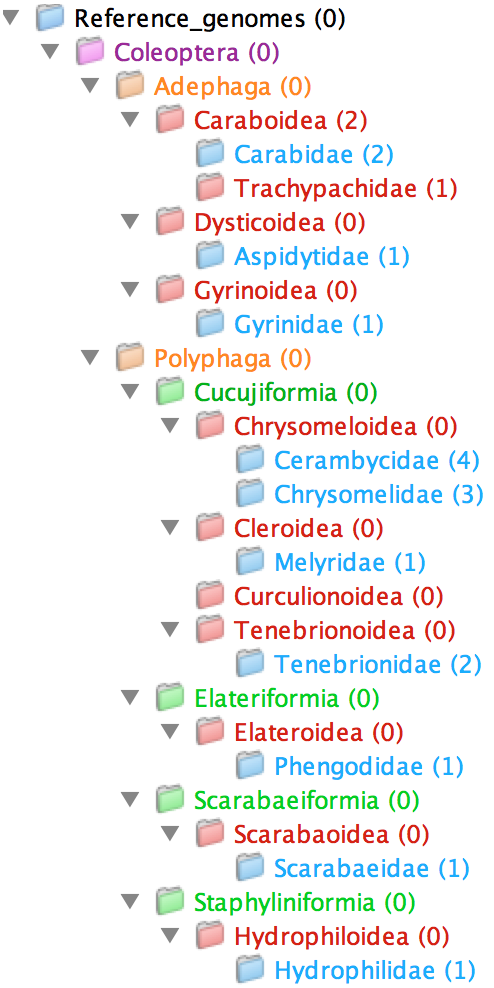
\includegraphics[width=0.25\textwidth]{blast5.png}%
\hfil
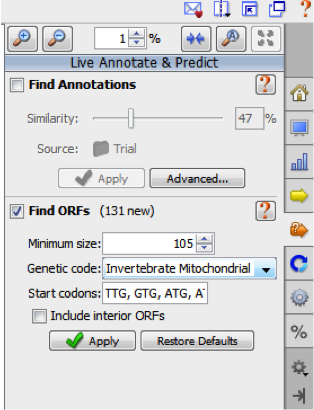
\includegraphics[width=0.35\textwidth]{LAP.png}%
}%\\[0.5cm] If you want some vertical space
  \captionof{figure}{\footnotesize Folders and the `Live Annotate \& Predict' toolbar}
  \label{fig:blast5}\label{fig:LAP}
\end{figure}

Our previously un-annotated sample mitochondrion now looks very busy. To make alignment clearer we can choose which annotations we want to be displayed. Access the `Annotation and Tracks' tool set by clicking on the yellow arrow above the `Live Annotate \& Predict' orange arrow pin. 
\\
\\
For our purposes we only want to see the gene, CDS and ORF options so unselect the other annotation types. We now have a roughly annotated mitochondrial sequence showing the important information~(\autoref{fig:ann3}). 


\begin{figure}[H]
  \centering
    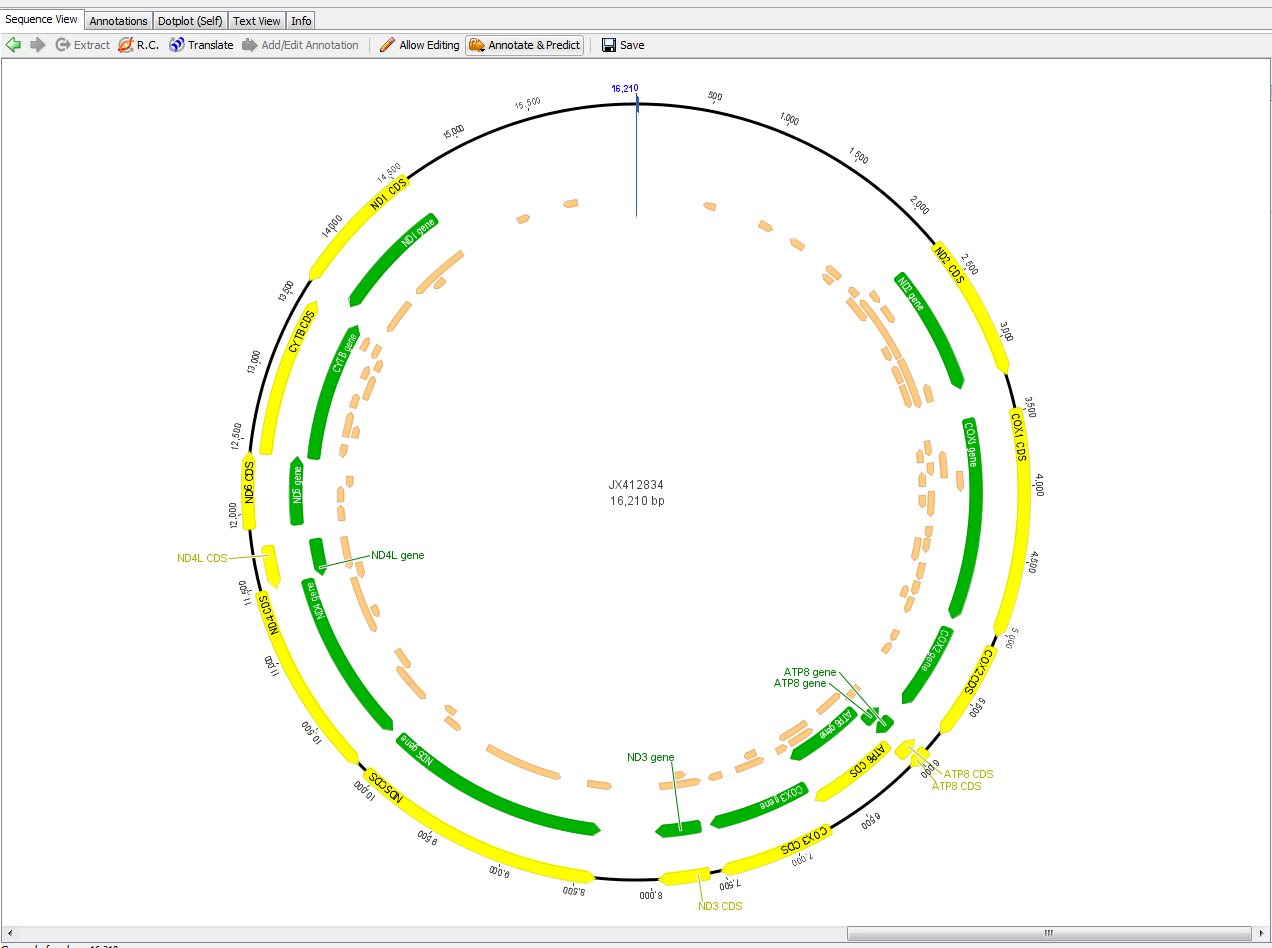
\includegraphics[width=0.8\textwidth]{ann3.png}
  \captionof{figure}{\footnotesize Roughly annotated mitochondrial sequence}
  \label{fig:ann3}
\end{figure}

\subsection{Edit Annotations}
Go to Annotations, select all and click Edit Annotations~(\autoref{fig:removeanno}). Select transl\_except and click Remove. Select note and click Remove. These are the translation exceptions from the previous references, which may not be applicable to our current supercontig.
\\
\\
The next step is to consider whether the annotations have been transferred accurately and that their position on the new mitochondrion makes biological sense i.e. within an ORF, starting with a methionine etc. In the `Display' tool set on the right, tick the Translation option and alter the frame to `By selection or annotation' and \textbf{set the genetic code to Invertebrate Mitochondrial: (transl\textunderscore table 5)}. This adds a track which allows us to see what amino acids any selected sequence codes for, particularly useful for identifying start and stop codons. At this point it is also advisable to change the sequence view from circular to linear using the sequence tab at the top of the Geneious window or the mapped keyboard shortcut (Ctrl+Shift+C). 
\\
\\
Click on the first gene ND2 CDS and zoom in (Zoom to selection: Ctrl+Shift+M). The imported annotation should start with a methionine. Edit each of the gene annotations such that they should start on a methionine (ATG, ATA, ATT, TTG, ATC) and end on a stop codon (TAA, TAG). Special cases for stop codons may occur~\secref{stopcodon}.

\subsection{Case Studies}

\subsubsection{Missing Gene Annotations}
\label{missinggene}
In cases where even with 25\% similarity, certain genes are missing, do the following steps. Create a folder with the missing gene name. For example, COX1. In many cases, despite blasting the COX1 gene to obtain the reference genome, the COX1 gene refuses to be transferred. We do not know why this is so. Nonetheless, click on the gene CDS from the reference genome and left click to Extract region. This will extract the COX1 gene into a new file. Transfer the new file into the COX1 folder. At the same time, extract COX1 gene regions from a multiple of other reference genomes that are found in the Reference genomes folder. Preferably, choose those that are closest in phylogeny to the Reference genome of the supercontig. 
\\
\\
After transferring a number of COX1 genes into the COX1 folder, go back to the `Live Annotate \& Predict' Toolbar~(\autoref{fig:LAP}) and click Find Annotations, choosing the COX1 folder as the source. Out of the numerous genes extracted, usually one would be able to be transferred. If none have a high enough similarity, extract a few more COX1 genes from other reference genomes and repeat the process. Choose the one with the highest similarity and click Apply. You can do the same for other missing genes, using one folder in the Stock References for each gene.

\subsubsection{Missing Start Codon}
Sometimes, the ORF indicates that the gene starts at another methionine and not the one indicated by the transferred gene annotation. The gene annotation may also not start at a methionine. In such cases, where you don't know whether to extend the COX3 gene, run a translated blast (blastx) of the longer candidate sequence (Genetic code = Invertebrate Mitochondrial (5), within the non-redundant protein sequnces database in NCBI) and then look at the length of the hits. Also you can look at the hit flanking sequences and compare this directly to the sequence in Geneious i.e. WGS highly conserved through the hits. This can then help you decide whether to extend or reduce the gene annotation.
\\
\\
Likewise, you can click on the longer candidate sequence and left click, selecting Translate... and click OK. Select the whole protein sequence and copy into blastp on NCBI website and run. If search times are becoming ridiculously long, under Organism in the BLAST options, type Coleoptera and select that taxa to make search timings much shorter. If no suitable start codon can be found, ensure that the starting amino acid is as similar in terms of properties to methionine as possible.

\subsubsection{Missing Stop Codon}
\label{stopcodon}
Similarly, if no Stop Codons are found, use the same method as that in Start Codons and blast the longer candidate sequence. Coleoptera genes can also end with a single T or TA. In such cases, double click the CDS which will produce a popup window~(\autoref{fig:addanno}). Ensure that you have deleted any transl\_except and notes transferred over from the reference genome. 

\begin{figure}[H]
  \centering
    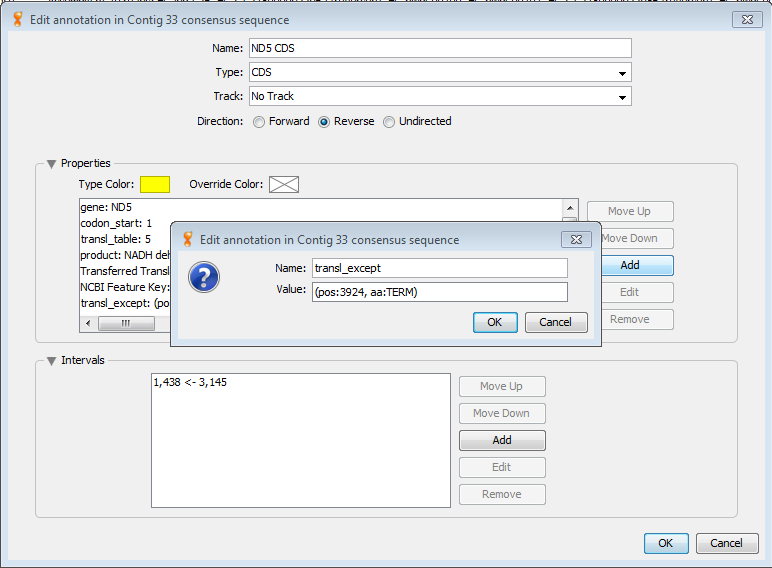
\includegraphics[width=0.6\textwidth]{addanno.png}
  \captionof{figure}{\footnotesize Adding Annotations}
  \label{fig:addanno}
\end{figure}

Click Add. Type the following for single T stop codons: 
\begin{displayquote}
Name: \textbf{transl\_except} \\
Value: \textbf{(pos:base position of T, aa:TERM)} \\
For example: Value: \textbf{(pos:3924, aa:TERM)} \\
If exception is on the reverse strand: Value: \textbf{(pos:complement(3924), aa:TERM)} \\
\end{displayquote}

For TA stop codons: 
\begin{displayquote}
Name: \textbf{transl\_except} \\ 
Value: \textbf{(pos:[smaller base position]..[larger base position], aa:TERM)} \\
For example: Value:\textbf{ (pos:3924..3925, aa:TERM)} \\
If exception is on the reverse strand: Value: \textbf{(pos:complement(3924..3925), aa:TERM)} 
\end{displayquote}
\begin{displayquote}
\footnotesize{*When submitting to GenBank, we have changed all TA stop codons to T stop codons as it was giving us a submission error of `Missing Stop Codon'. We have no idea why~\frownie.} \\
\end{displayquote}

Click OK. Add another annotation by clicking Add and type the following: 
\begin{displayquote}
Name: \textbf{note} \\
Value: \textbf{TAA stop codon completed by the addition of 3'A residues to the mRNA} 
\end{displayquote}

If at anytime you are unsure of anything, select the sequence and click Add annotation. Key in the problem in the Name, for exampe, ND3 no stop, and click OK. This allows you to come back to be problem easily and also to delete all annotations of the misc\_feature type after clarifying all problems~(\autoref{fig:misc}).

\begin{figure}[H]
  \centering
    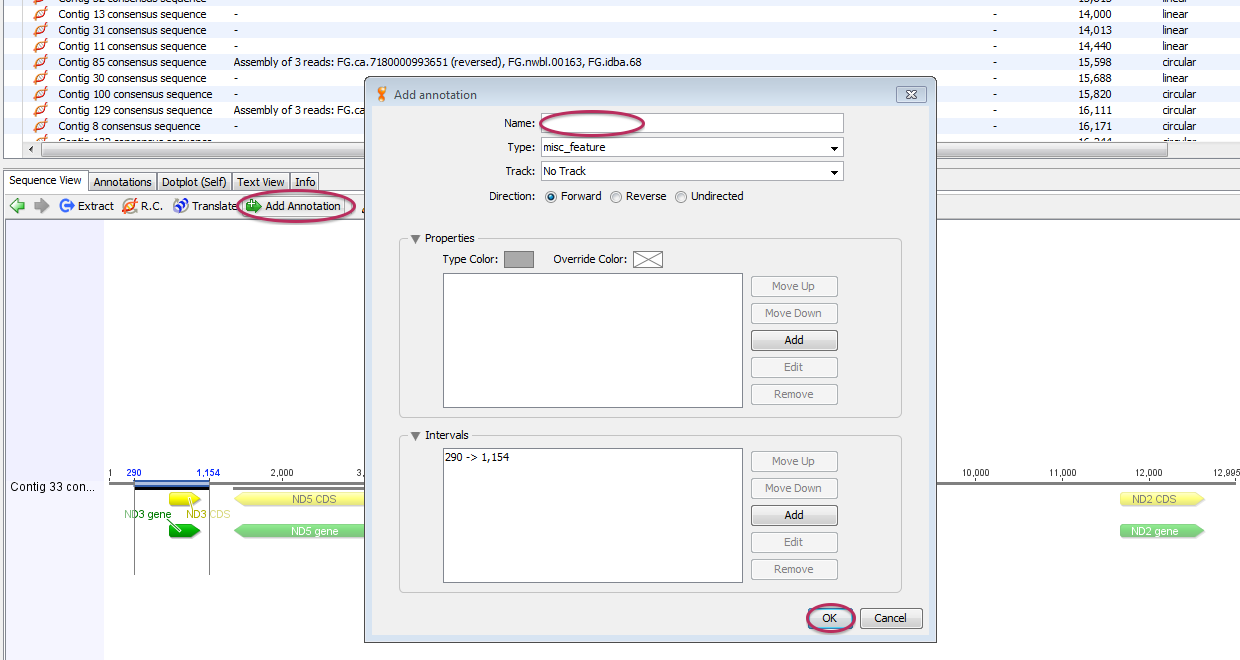
\includegraphics[width=0.9\textwidth]{misc.png}
  \captionof{figure}{\footnotesize Adding misc\_feature}
  \label{fig:misc}
\end{figure}

\subsection{Removing Annotations}
\label{subsec:Removing}
Select all supercontigs and click Annotations. Select all annotations and click on Edit Annotation which is beside a green arrow~(\autoref{fig:removeanno}). A pop-up window will appear. Select and click Remove to delete protein\_id, db\_xref, Transferred from, Transferred similarity, Translation. Also remove all Annotations that has Type: Source, misc\_feature or tRNA. Delete also other random things that only appear for one supercontig and not the rest, for example Transferred Translation.

\begin{figure}[H]
  \centering
    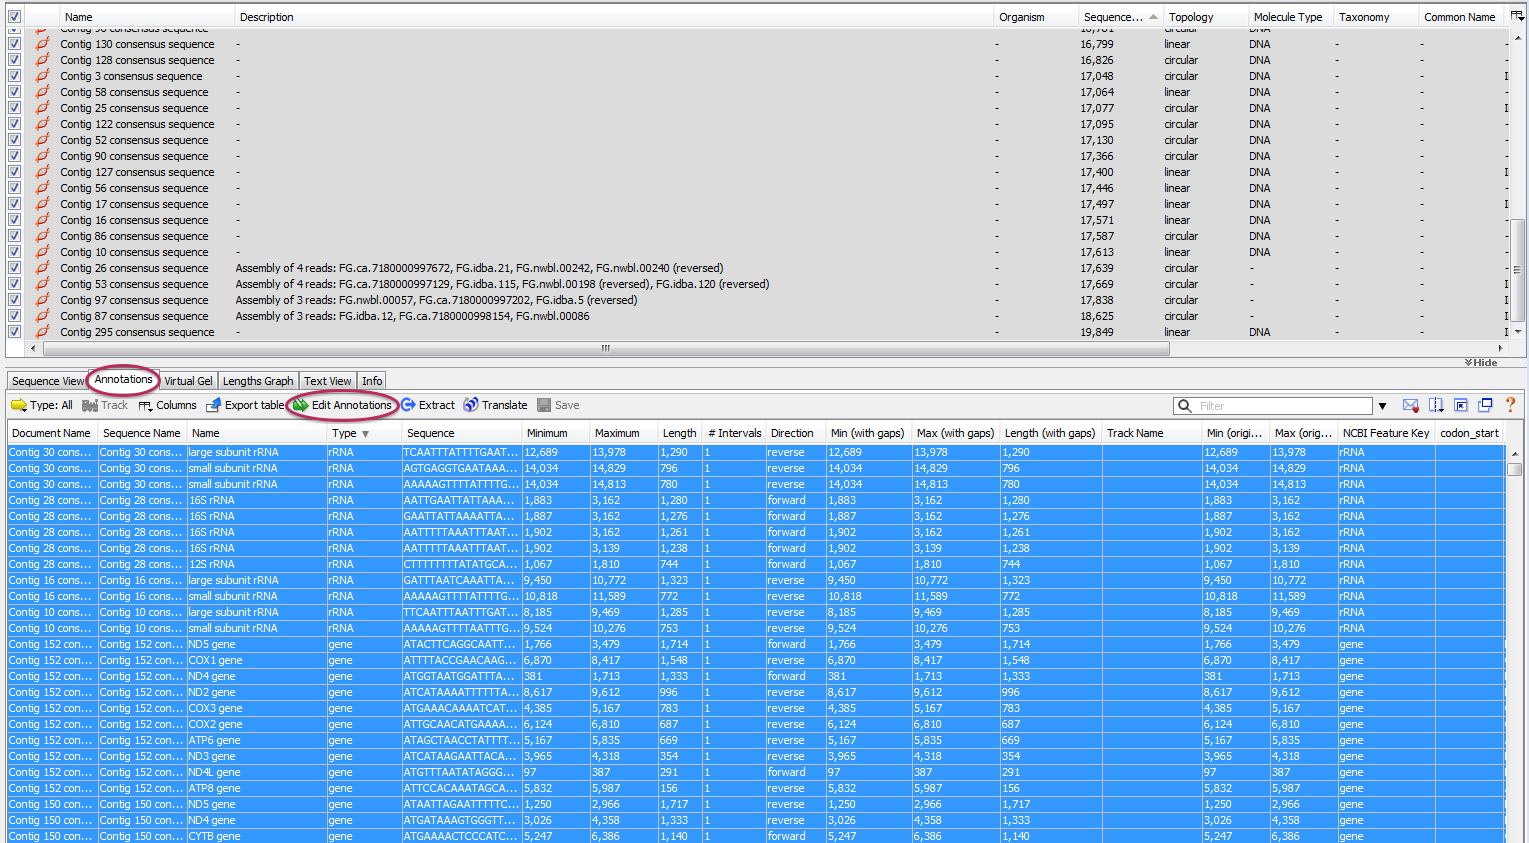
\includegraphics[width=0.9\textwidth]{removeanno.png}
  \captionof{figure}{\footnotesize Removing Annotations}
  \label{fig:removeanno}
\end{figure}

\subsection{Keeping a datasheet}
Keeping a datasheet of the annotation process will give us further insight into the genes. BlastGene referred to the gene from the supercontig that we used for Blast. ReferenceGenome refers to the genome from which the annotations were transferred. Superfamily referred to the superfamily of the ReferenceGenome~(\autoref{fig:annodatasheet1}). 
\\
\\
Number of bases we extended or reduced the transferred annotations by were recorded under GeneBP by a positive number and a negative number respectively and the stop and start codons were recorded as well. An `!' was used when we could not find a start or stop codon and NA was used when the sequence is too short and hence did not have the indicated genes~(\autoref{fig:annodatasheet2}). 
\\
\\
\begin{figure}[H]
  \centering
    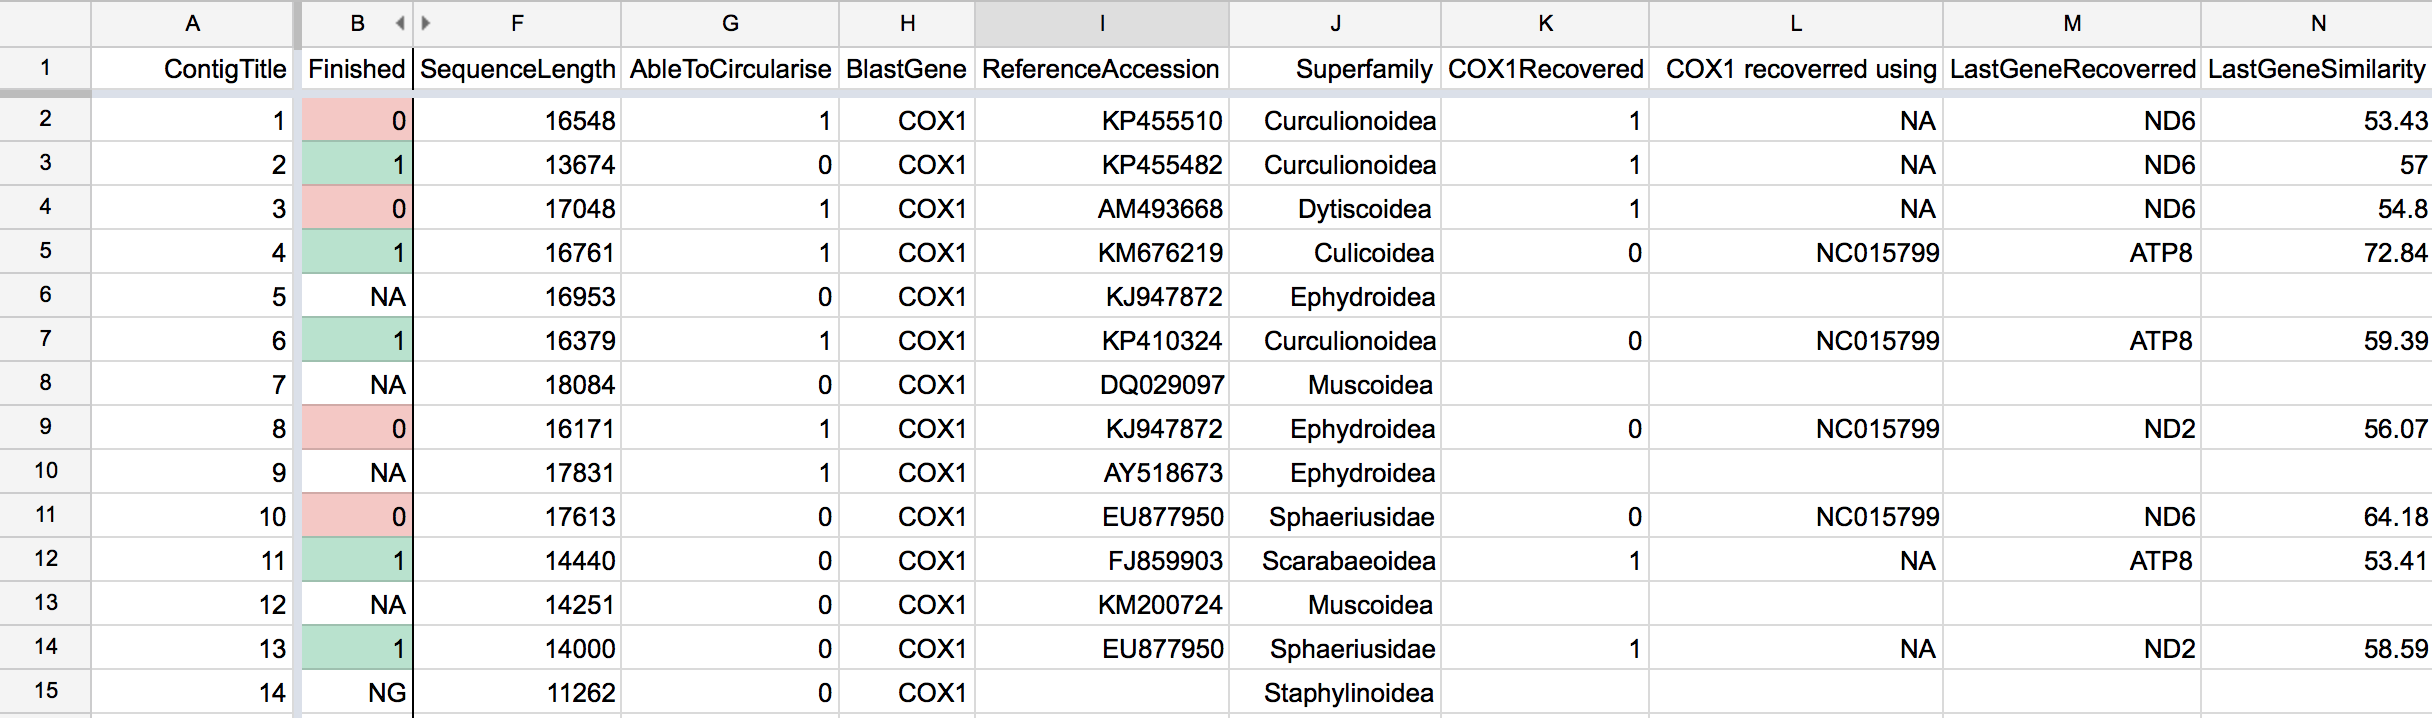
\includegraphics[width=\textwidth]{annodatasheet1.png}
  \captionof{figure}{\footnotesize Recording Annotation Edits}
  \label{fig:annodatasheet1}
\end{figure}

\begin{figure}[H]
  \centering
    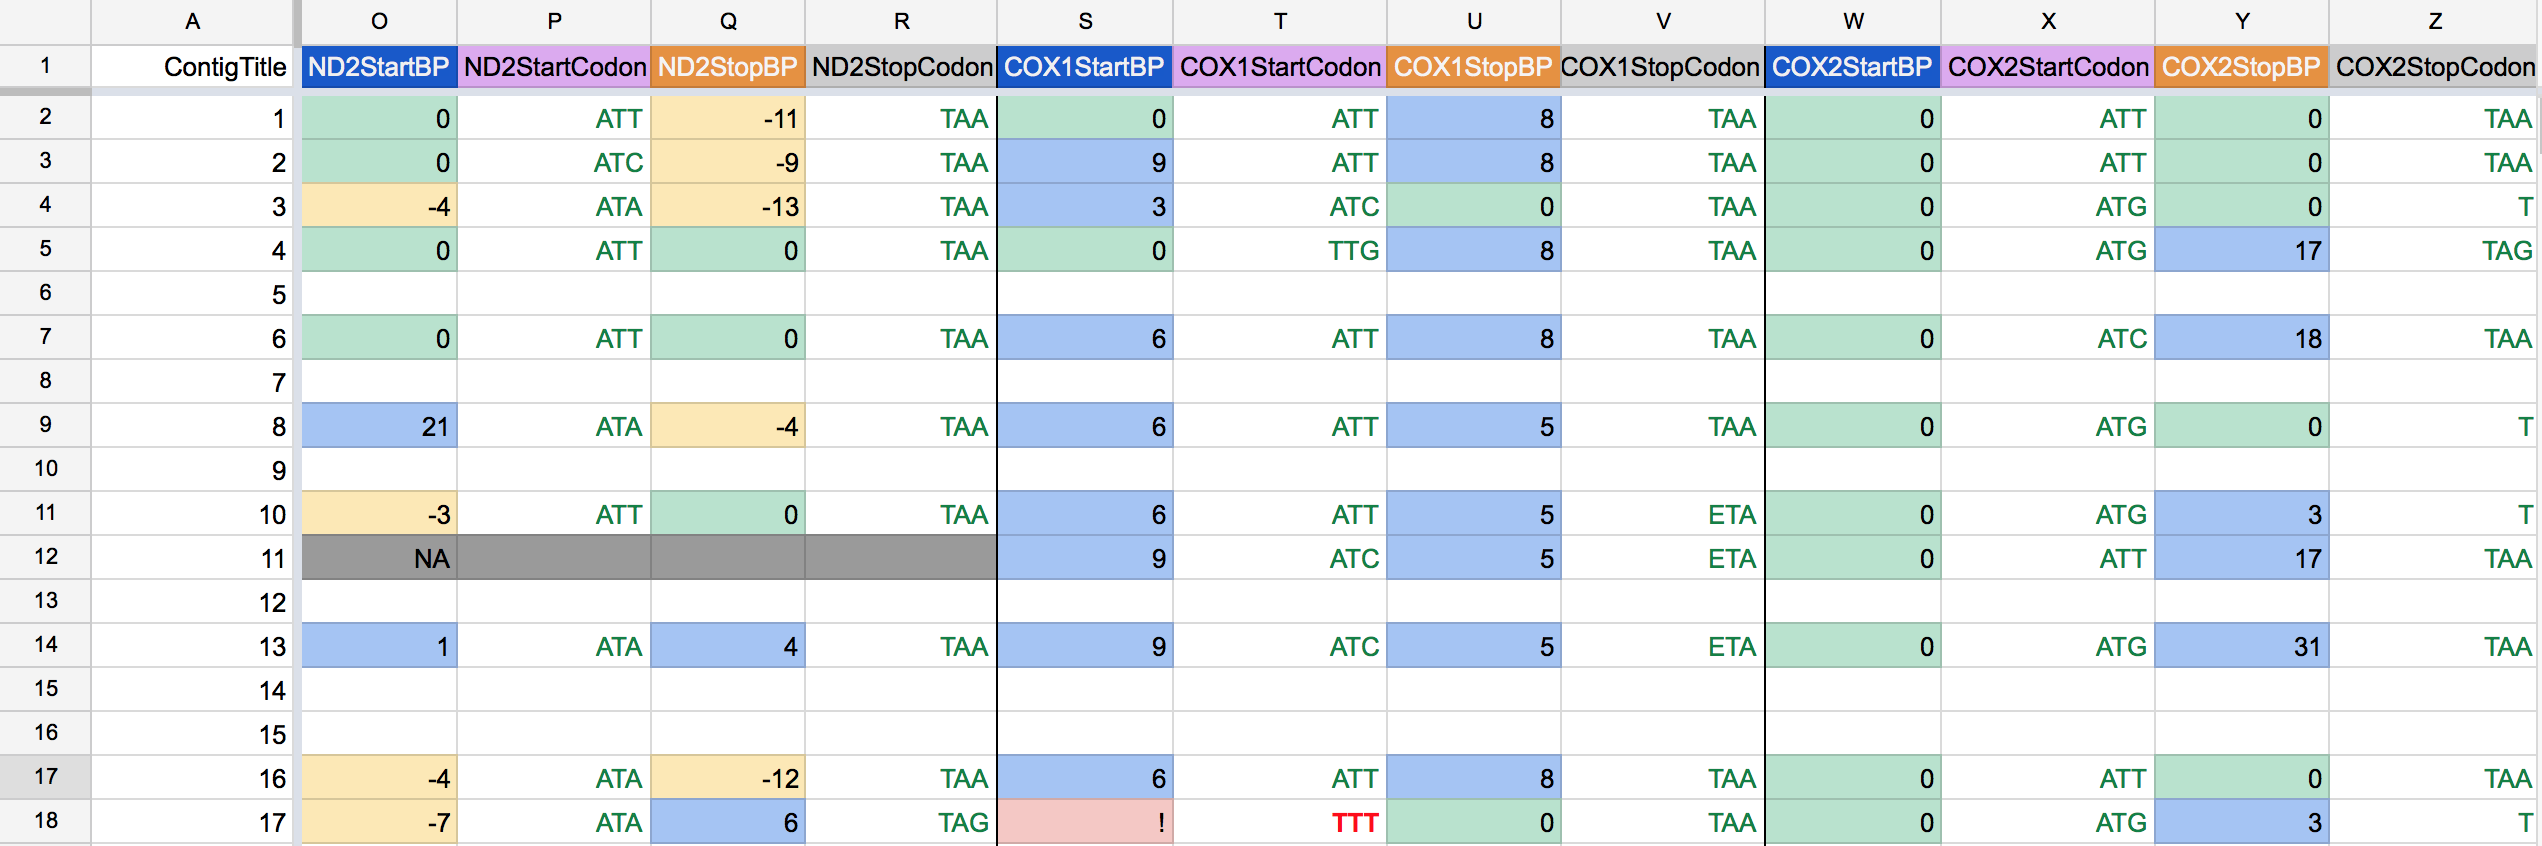
\includegraphics[width=\textwidth]{annodatasheet2.png}
  \captionof{figure}{\footnotesize Recording Annotation Edits}
  \label{fig:annodatasheet2}
\end{figure}
\hfill \break

Using these data, we could also create diagrams in R to show common trends~(\autoref{fig:fgstart}, \autoref{fig:fgstop}, \autoref{fig:fgstartbp}, \autoref{fig:fgstopbp}).

\begin{figure}[H]
  \centering
    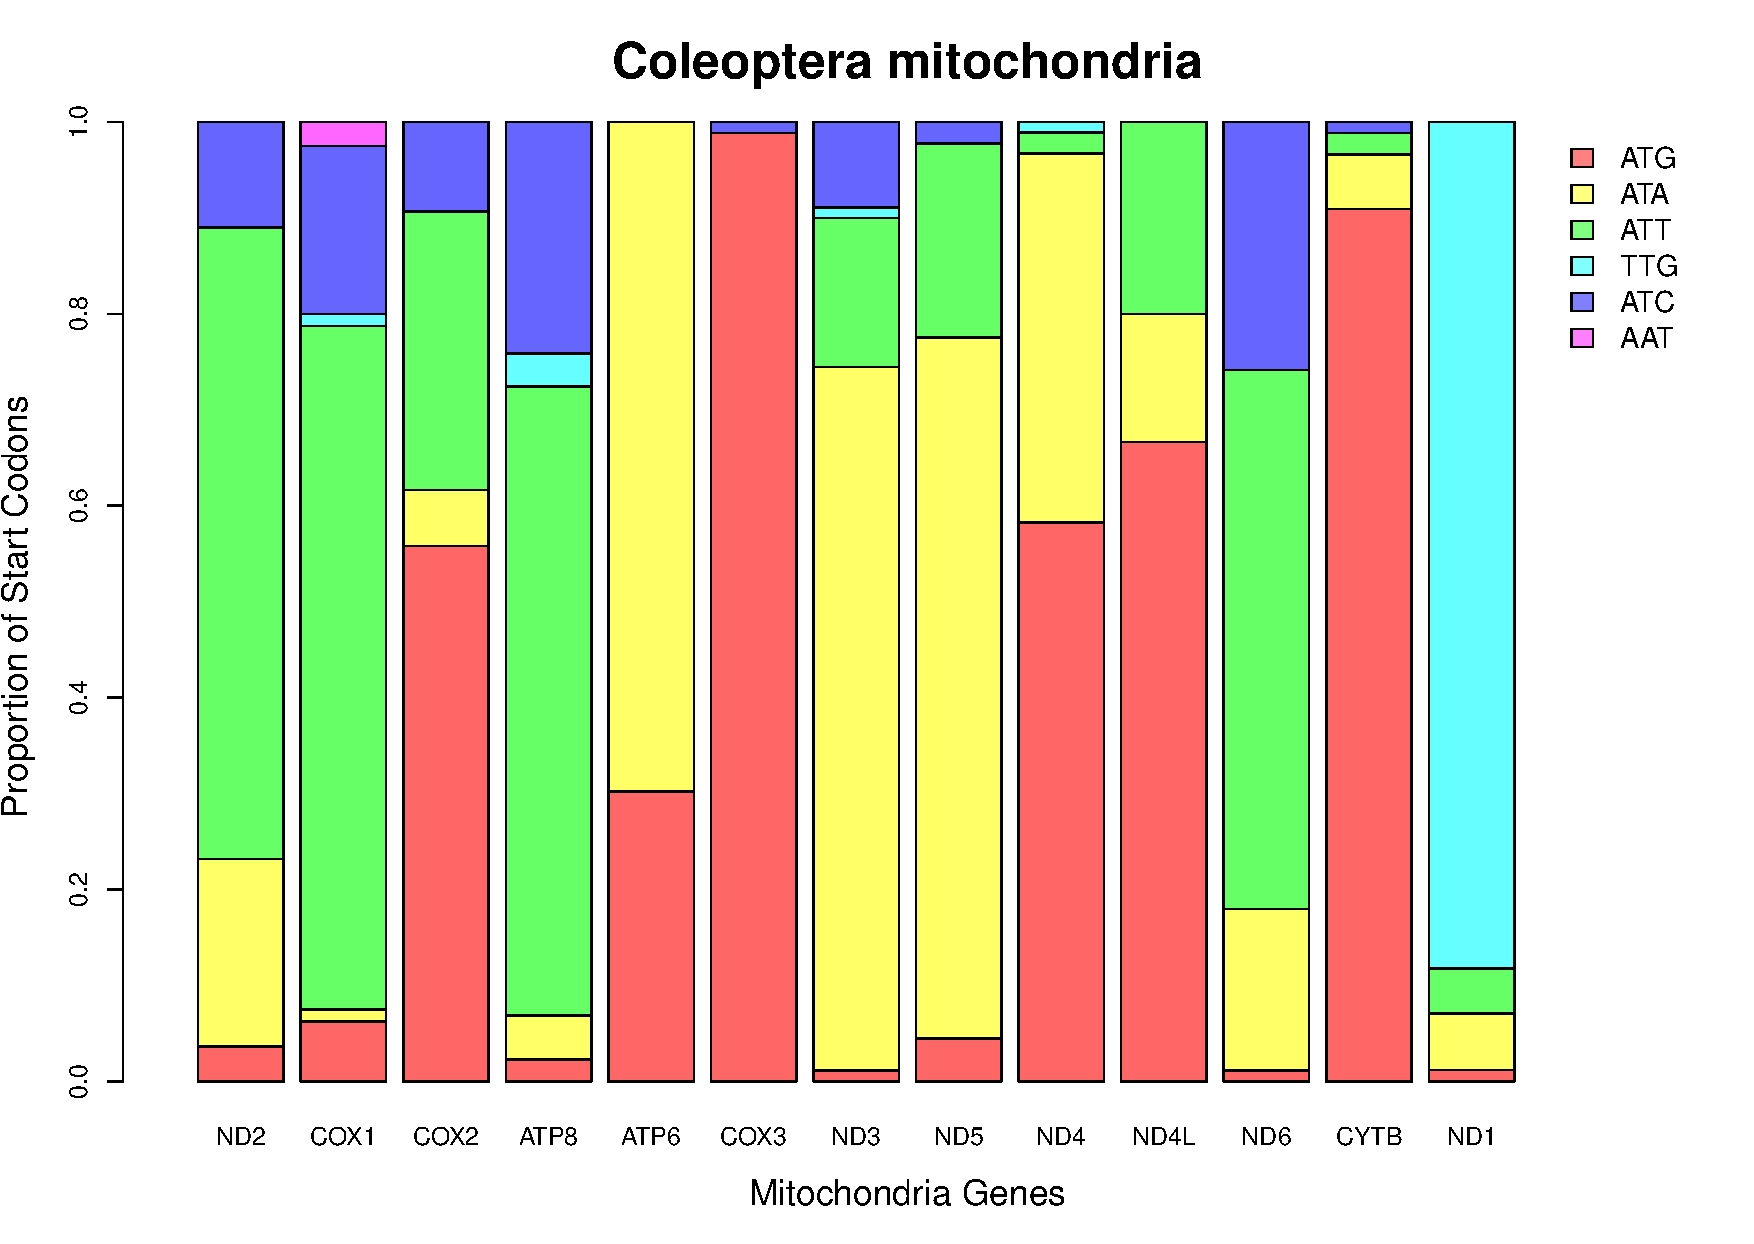
\includegraphics[width=0.95\textwidth]{fgstart.pdf}
  \captionof{figure}{\footnotesize Start codons of mitochondrial genes.}
  \label{fig:fgstart}
\end{figure}

\begin{figure}[H]
  \centering
    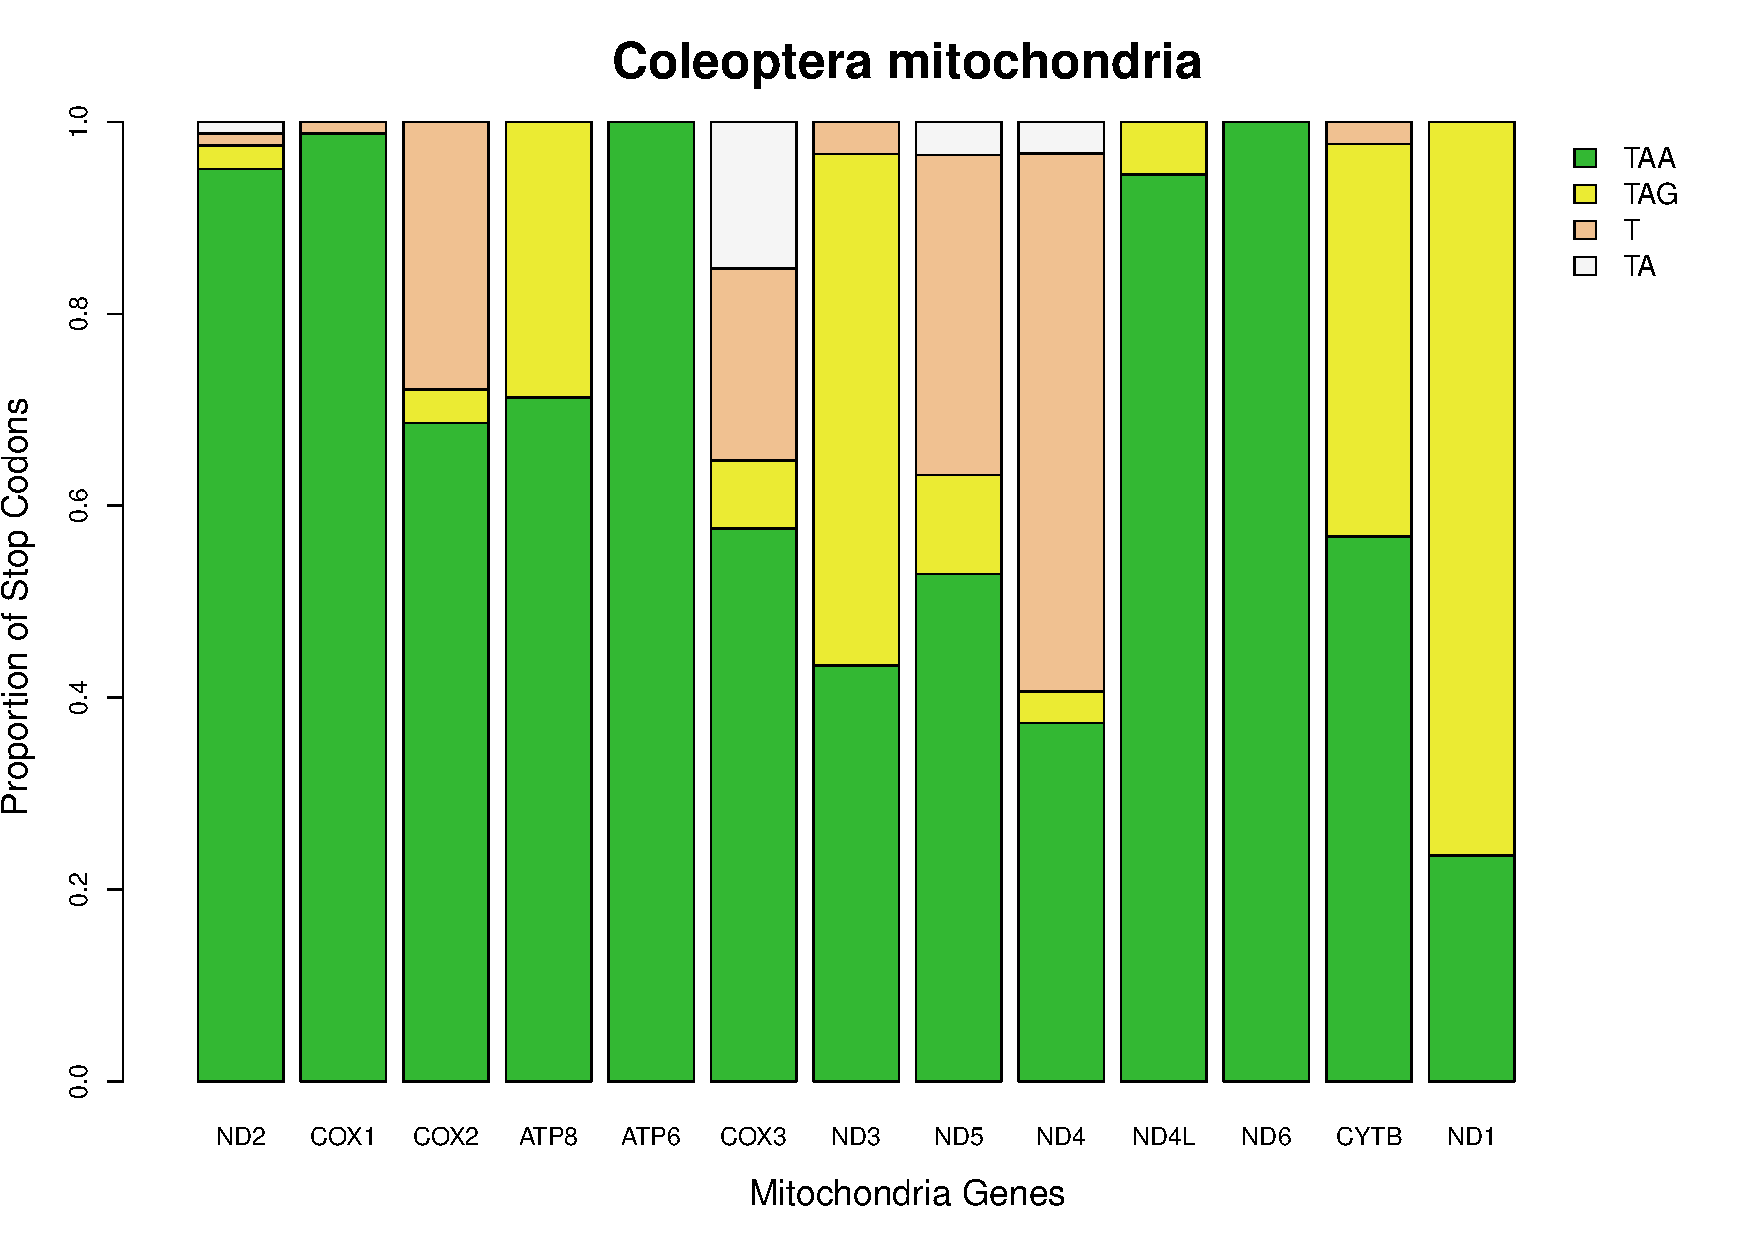
\includegraphics[width=0.95\textwidth]{fgstop.pdf}
  \captionof{figure}{\footnotesize Stop codons of mitochondrial genes.}
  \label{fig:fgstop}
\end{figure}

\begin{figure}[H]
  \centering
    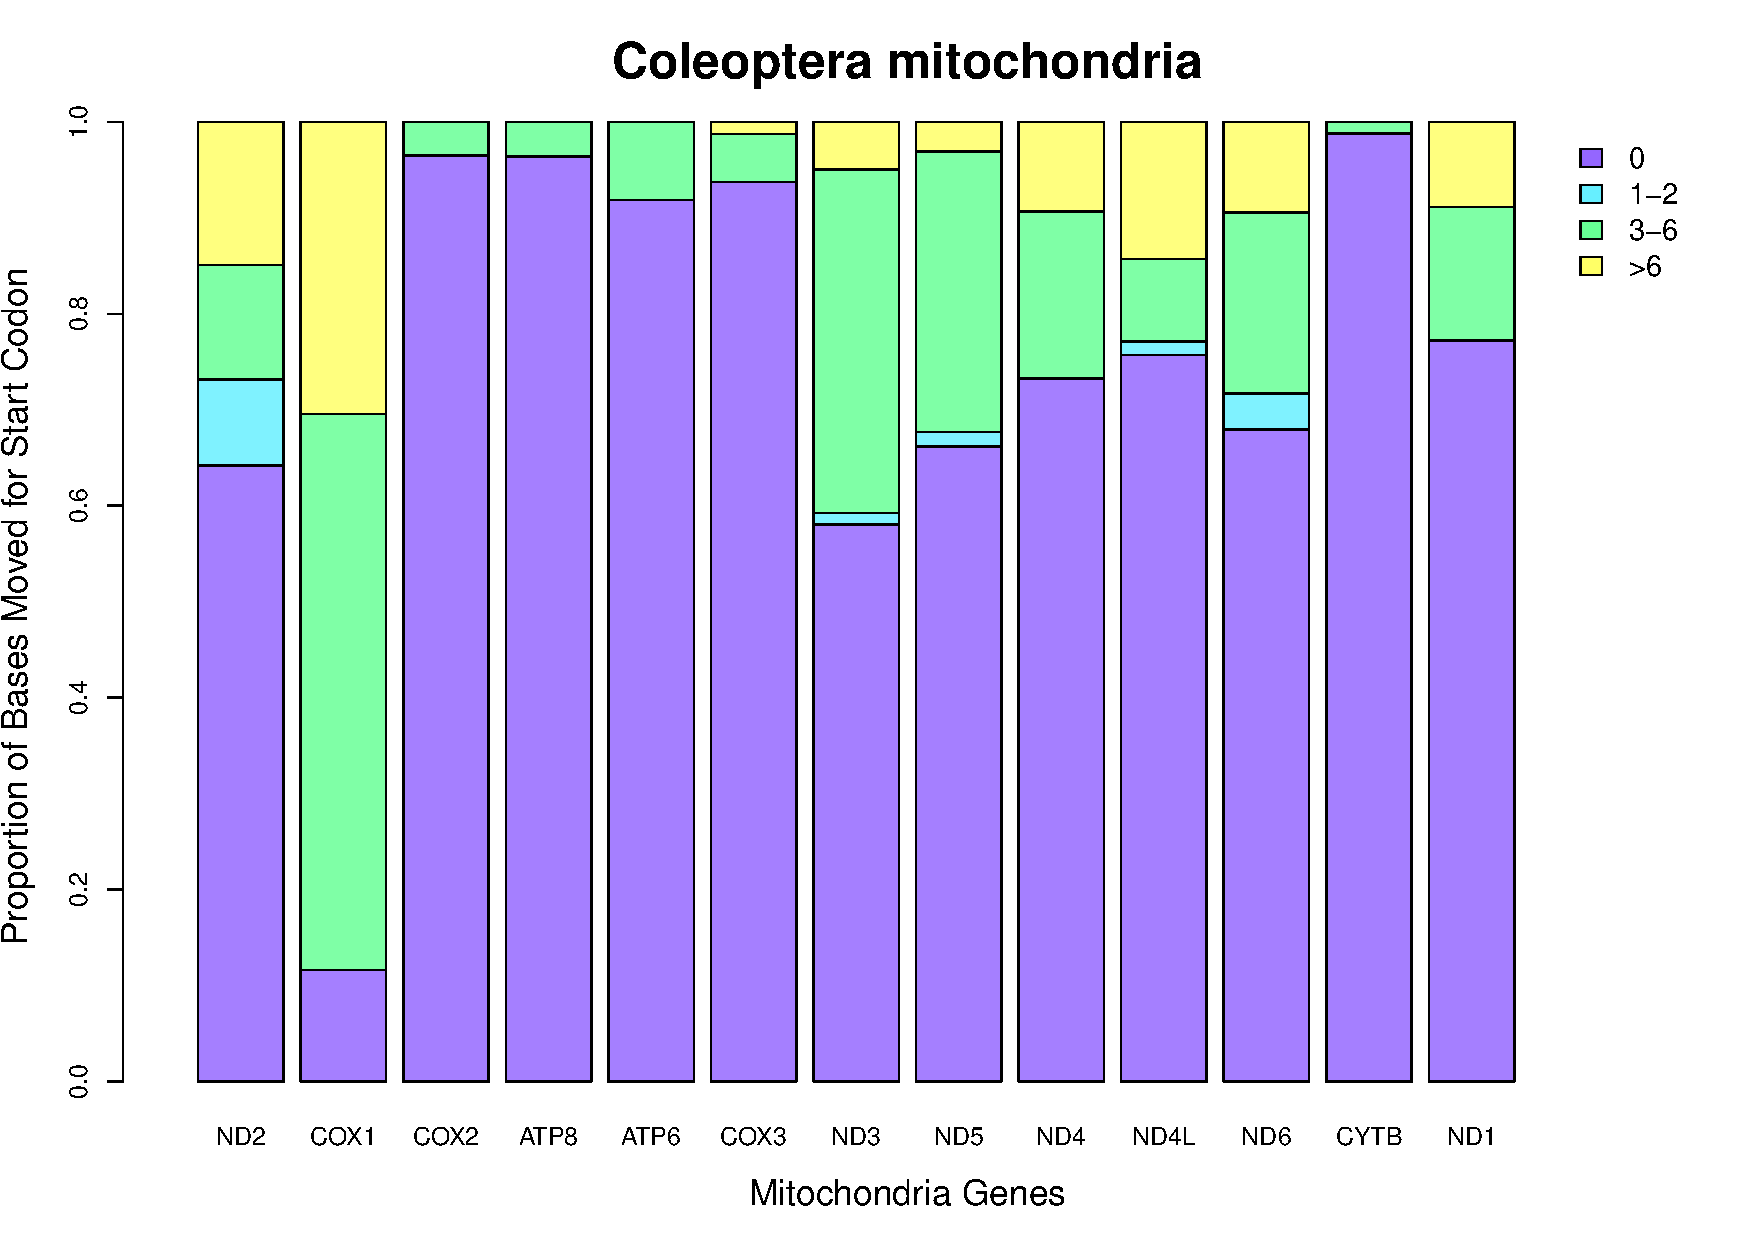
\includegraphics[width=0.95\textwidth]{fgstartbp.pdf}
  \captionof{figure}{\footnotesize Number of bases moved in editing start codons of mitochondrial genes.}
  \label{fig:fgstartbp}
\end{figure}

\begin{figure}[H]
  \centering
    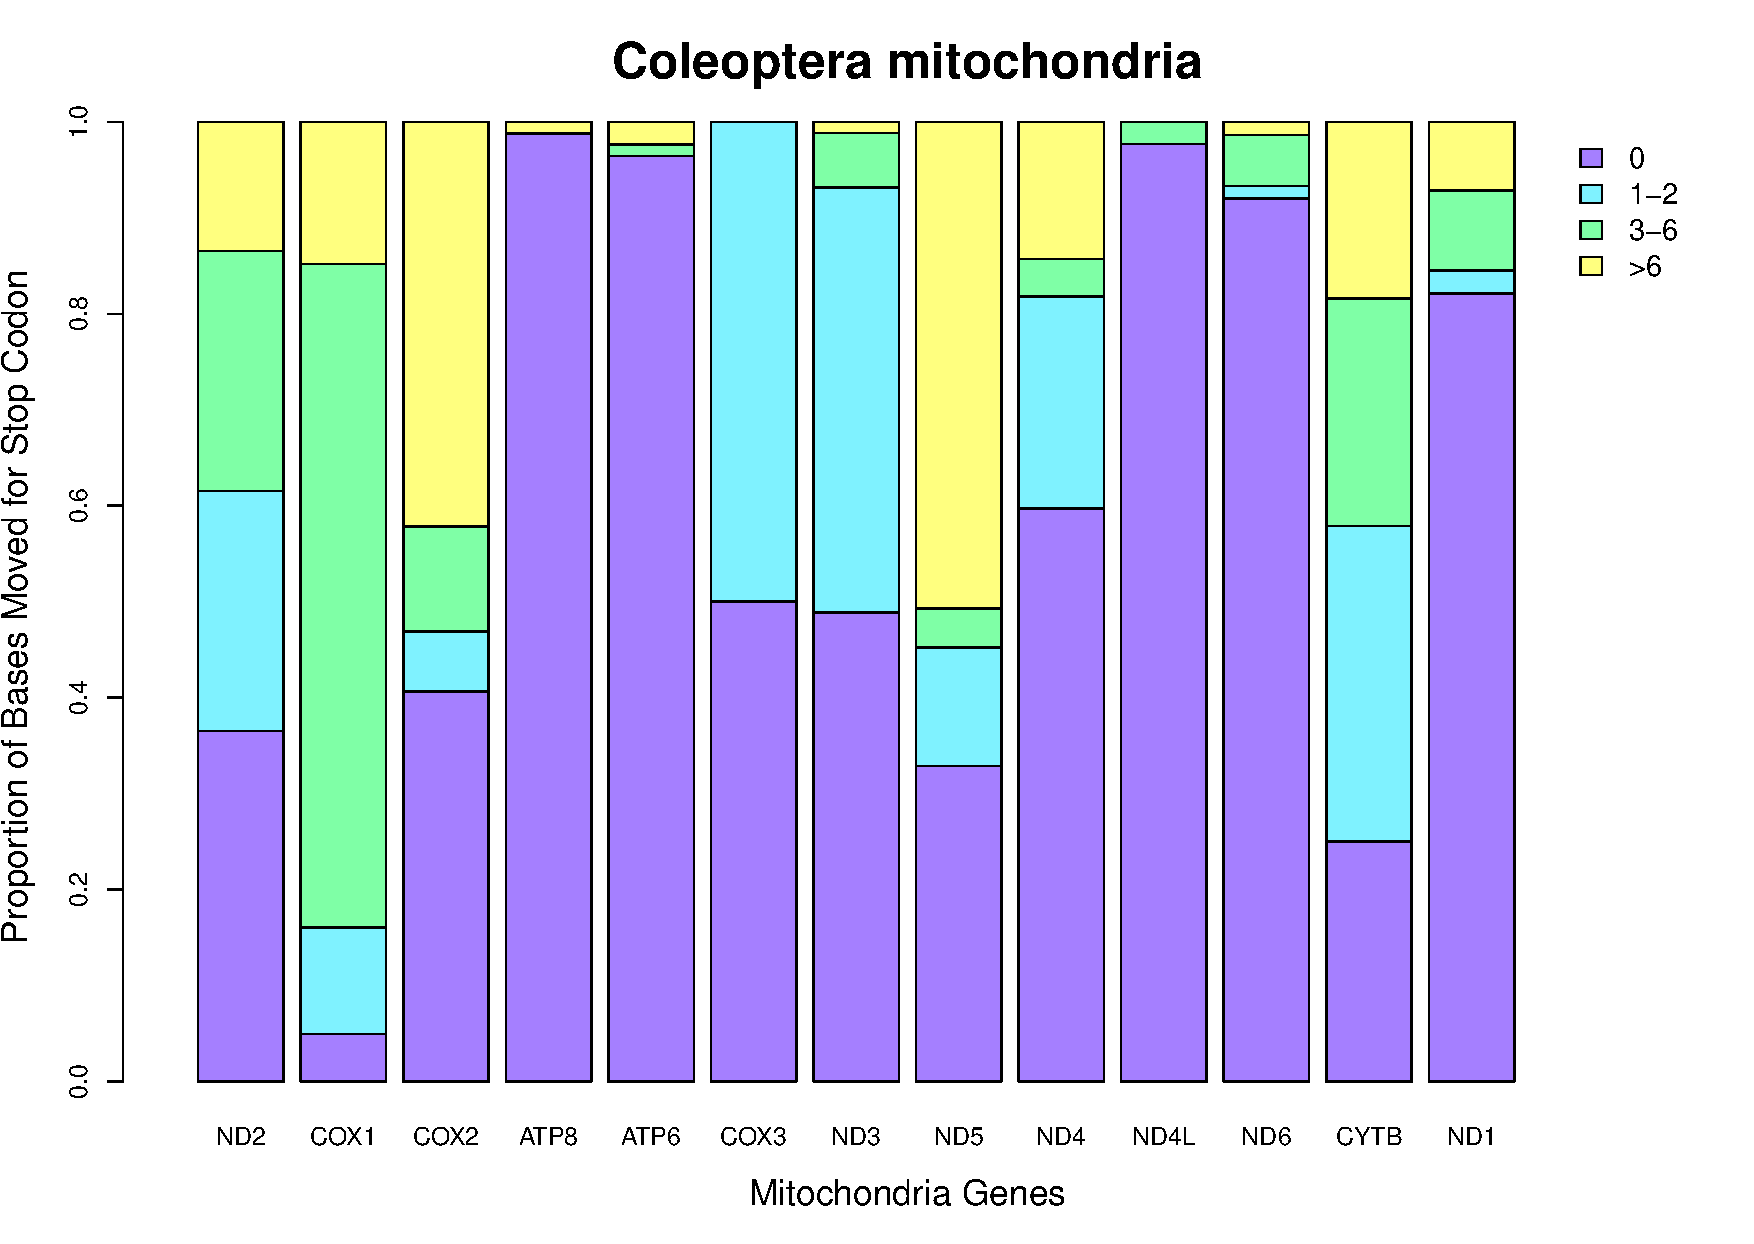
\includegraphics[width=0.95\textwidth]{fgstopbp.pdf}
  \captionof{figure}{\footnotesize Number of bases moved in editing stop codons of mitochondrial genes.}
  \label{fig:fgstopbp}
\end{figure}

\newpage
\section{Adding tRNAs}
\label{sec:Adding}
To add tRNA annotations, first delete all existing tRNA annotations if you have not already done so. 
\\
\\
Refer to `My time-saving COREALLA' guide. For Windows, download Filezilla portable and Putty. For Mac users, download Cyberduck. Filezilla and Cyberduck allow you to transfer files to and from the server easily. After obtaining your username and password from Benjamin, log on to ctag. Transfer the startup kit from ben's directory into your directory. 
\\
\\
Export all the consensus sequences into one fasta file and upload it into the tRNA folder using Cyberduck or Filezilla. Set your directory into the tRNA stuff folder by using the cd command which should look somewhat like this:
\begin{displayquote}
cd starter\textbackslash kit/tRNA\textbackslash stuff/ \\
\end{displayquote}

Run the following commands:
\begin{displayquote}
perl all2many.pl [filename] 1000 \\
sh covel\_wrap\_multithread.sh
\end{displayquote}
\begin{displayquote}
\footnotesize*You have to allocate memory (15 or 20)
\end{displayquote}

\begin{displayquote}
perl covels\_wrap.pl. 
\end{displayquote}
\begin{displayquote}
\footnotesize*This script will take a long time to run. To run it overnight, refer to the `My time-saving COREALLA'.
\end{displayquote}

\begin{displayquote}
perl cove\_output20130710.pl
\end{displayquote}
\begin{displayquote}
\footnotesize*This will generate a folder called GB and in it is the .gb file which you can transfer back into Geneious. \\
\end{displayquote}

Select all of your original supercontigs and the ones with tRNAs on it. Go to Tools, Align/Assemble, De Novo Assemble... If your files all start with the same format, Tick Assembly by 1st or 2nd part of name to make the process easier and leave other options as default. It is recommended to assemble by name. 
\\
\\
If the names are separated by different things, for example the one by tRNA is by \_ and the original supercontigs by a space, this will not work. If you do not assemble by name, Geneious will reorder the supercontigs and it becomes hard to track which supercontig comes from where. Otherwise, you can chnage the supercontig names manually after assembly.
\\
\\
There should be no unused reads. If there are, something somewhere has gone wrong. Recheck your sequences and tRNA annotations.
\\
\\
After assembly is done, place the Assembly report and Consensus Sequences into another folder. Select all the assembled new supercontigs and go to Annotate \& Predict at the top menu bar, Transfer Annotations and follow through. As the sequences are all identical, you do not have to do it manually. Thereafter, you should see that the consensus sequence contains both the annotations that you have manually edited as well as the new tRNA annotations~(\autoref{fig:tRNA}). 
\\
\\
Check through all the consensus sequences and ensure that they all have the transferred annotations. Remove any generated unneeded annotations~(Refer to \autoref{subsec:Removing}).

\begin{figure}[H]
  \centering
    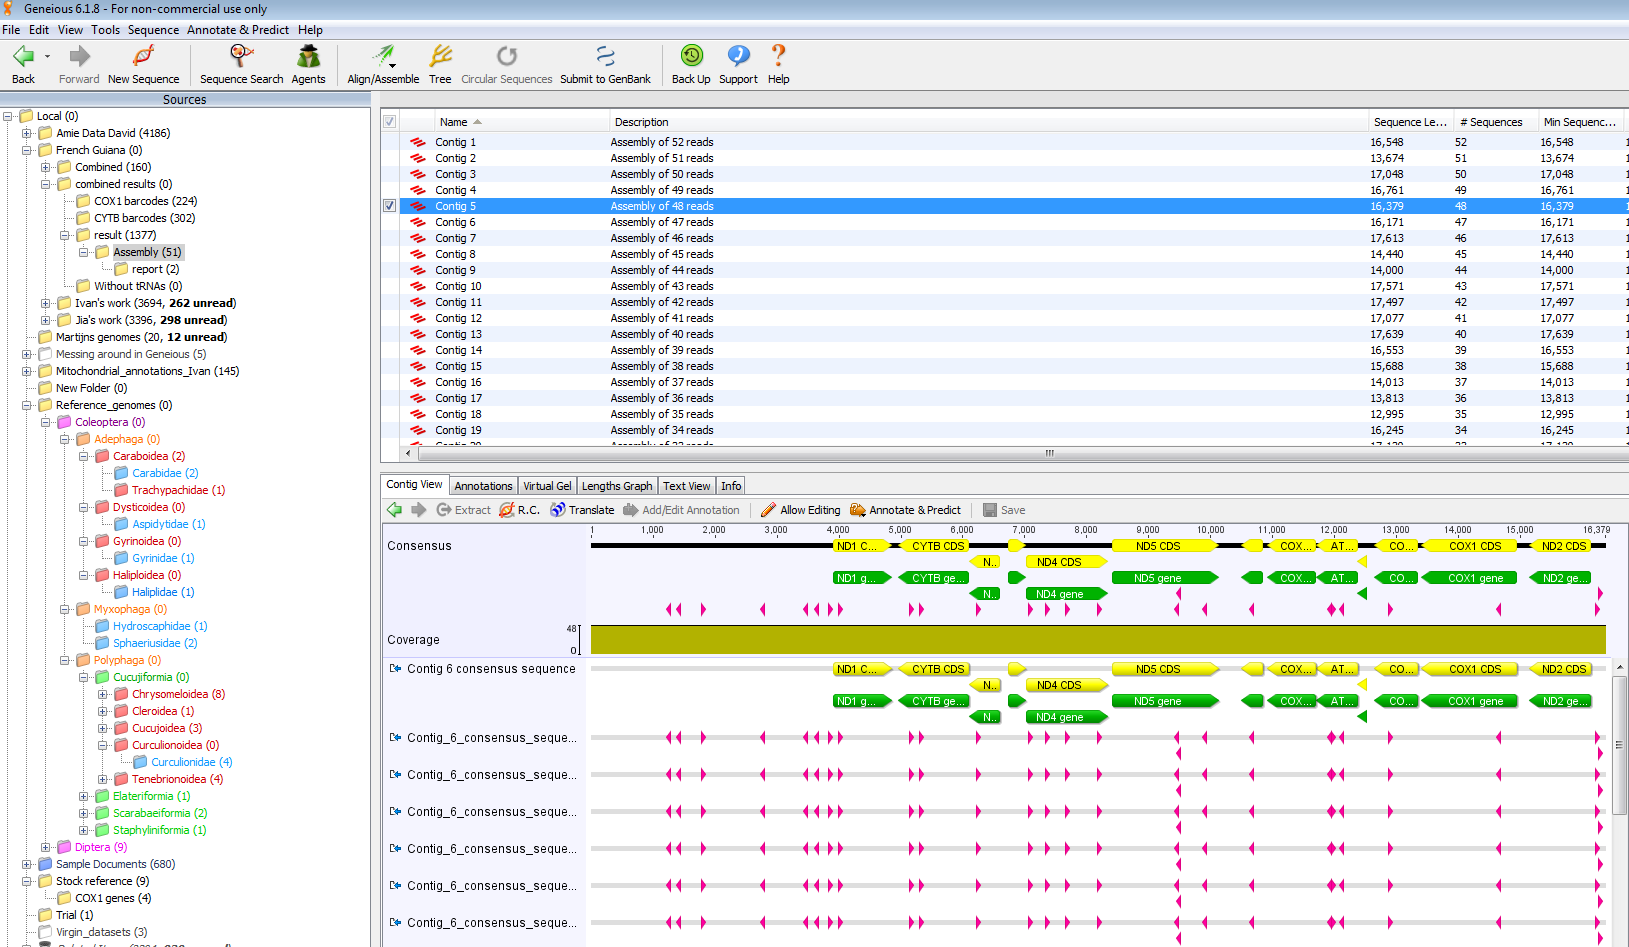
\includegraphics[width=0.9\textwidth]{tRNA.png}
  \captionof{figure}{\footnotesize Transferring tRNA annotations.}
  \label{fig:tRNA}
\end{figure}

A complete circular mitochondrion should ideally have 22 tRNAs as beautifully demonstrated in \exautoref{fig:tRNA2}.

\begin{figure}[H]
  \centering
    \includegraphics[width=0.93\textwidth]{tRNA2.png}
  \captionof{figure}{\footnotesize Consensus sequence with all 22 tRNA annotations.}
  \label{fig:tRNA2}
\end{figure}

If any tRNA or rRNA annotations are missing, create a folder called tRNA annotations. Create a copy of one of the reference genomes with 22 tRNA annotations downloaded. Click on Annotations of the copy of reference genome. Select all non-tRNA and non-rRNA annotations and press Delete. You should be left with all tRNA and rRNA annotations as seen in \exautoref{fig:tRNA3}. This step is similar to that in Section \ref{subsec:Removing}.

\begin{figure}[H]
  \centering
    \includegraphics[width=0.93\textwidth]{tRNA3.png}
  \captionof{figure}{\footnotesize Reference genome with only tRNA and rRNA annotations.}
  \label{fig:tRNA3}
\end{figure}

Place the file in the tRNA annotations folder. Go back to your consensus sequences with missing tRNAs. Select one of the consensus sequences. Click on Find Annotations in the `Live Annotate \& Predict' toolbar~(\autoref{fig:LAP}) but choose your tRNA annotations folder under Source. Select a high similarity of around 70\%. Ensure that all tRNA or rRNA annotations that are missing are present in the right location by comparing it to \exautoref{fig:tRNA2}. Click Apply. Remove any duplicated tRNA or rRNA annotations that have been transferred over. Your Sequence View should now look similar to \exautoref{fig:tRNA2} and have 22 tRNAs. This step is similar to that in Section \ref{subsec:Transferring}. 
\\
\\
You can now prepare your files for submission to GenBank.

\newpage
\section{Submitting to GenBank}
\label{sec:Submitting}
After barcoding, the process is not yet over. There are a few ways of submitting sequences. Geneious is one of the methods. However, it provides little flexibility and is a rather tedious process. The metadata of the project, such as the organism name and taxa, has to be keyed in for every consensus sequence individually. The other method that we have chosen to use is through tbl2asn.

\subsection{Submitting using Geneious.}
Go to Tools, Submit to GenBank in Geneious to reach the window below~(\autoref{fig:genbank}).

\begin{figure}[H]
\makebox[\textwidth]{%
\includegraphics[width=0.48\textwidth]{genbank.png}%
\hfill    
\includegraphics[width=0.48\textwidth]{genbank2.png}%
}%\\[0.5cm] If you want some vertical space
  \captionof{figure}{\footnotesize Submitting to Genbank in Geneious}
  \label{fig:genbank}
\end{figure}

Fill in the appropriate information. Select remove when asked if it is alright to remove unneccessary annotations. Usually, if not always, errors will appear~(\autoref{fig:genbank}). Below are some of the errors and methods of removing them~(\autoref{tab:errors}).

\begin{table}[H]
\centering
\captionof{table}{Errors and solutions to Submit to Genbank in Geneious.}
\label{tab:errors}
\begin{tabular}{|l|l|}
\hline
\rowcolor[HTML]{CBCEFB} 
Errors & Solutions \\ \hline
`given protein length does not match translation length' & Delete annotation of type `translation' \\ \hline

\multicolumn{1}{|l|}{`code-break location not in coding region'}  & \multicolumn{1}{l|}{\begin{tabular}[c]{@{}l@{}}Delete incorrect annotations \\ with feature `transl\_except'\end{tabular}}  \\ \hline

`anti-codon location.../unparsed anti-codon' & Delete annotation of type `anticodon' \\ \hline

\multicolumn{1}{|l|}{`Missing stop codon'}  & \multicolumn{1}{l|}{\begin{tabular}[c]{@{}l@{}}Change transl\_except of TA to only T \\ For ex. (pos:9559..9560, aa:TERM) to  \\ (pos:9559, aa:TERM). \end{tabular}}  \\ \hline

\multicolumn{1}{|l|}{`Inconsistent taxnames'}  & \multicolumn{1}{l|}{\begin{tabular}[c]{@{}l@{}} Change name of file to organism name\\ such that the description is the same as name. \end{tabular}}  \\ \hline

\end{tabular}
\end{table}


\subsection{Submitting using tbl2asn.}
In our internship, we decided to use tbl2asn instead, as it allows us to submit many sequences at once. You require three files for tbl2asn: the template file, fasta file and the feature table file. For more information about tbl2asn and the three files needed to generate a .sqn file, go to \url{http://www.ncbi.nlm.nih.gov/genbank/tbl2asn2/}. A summary of steps is found below~(\hyperref[pdf:template]{Refer to PDF diagram}).

\subsubsection{Generating the template file.}
\label{subsubsec:template}
You require the following information for the template file: the project title, sequence authors and publication status. Go to \url{http://www.ncbi.nlm.nih.gov/WebSub/template.cgi} and key in the required details and click Create template. This should generate the template file with suffix \textcolor{orange}{.sbt}. Take note that special characters such as \"{A} and \ss~are unfortunately not accepted in author names.


\subsubsection{Generating the fasta file.}
\label{subsubsec:fasta}
Ensure that the name of sequences is \textcolor{red}{BMNH number}\_(anything you like~\smiley). For ex. \\ 
1234567\_consensus\_sequence. Choose all sequences to be submitted and go to File, Export... in Geneious. Select FASTA(*.fasta) file type before saving the file. 
\\
\\
Check that the title of every sequence in the fasta file shows \textgreater\textcolor{red}{BMNH number}\_(anything you like~\smiley) and that the \textcolor{red}{BMNH number} corresponds with the title in the feature table file: \textgreater Feature\_\textcolor{red}{BMNH number}. For example, \textcolor{purple}{\textgreater1234567\_consensus\_sequence} in the fasta file should correspond with \textcolor{purple}{\textgreater Feature\_1234567} in the feature table file. If it does not match, the script to generate the complete fasta file will not work. Ensure that title is separated by a \_ and not by spaces or any other character. If they are, simply do a search for the character and replace with `\_' in the fasta file before running it with Benjamin's Script. 
\\
\\
Before running Benjamin's Script, compile a excel sheet with the following information: BMNH, the species name, the topology of the sequence(circular or linear), country and isolation\_source(method of collecting organism)~(\autoref{tab:bencsv}). Save the file as a Comma Separated Values(*.csv) file. It is crucial that under organism: Family name, sp., BMNH and number are separated by exactly one space.

\begin{table}[H]
\centering
\captionof{table}{CSV file to generate Fasta file.}
\label{tab:bencsv}
\begin{tabular}{|l|l|l|l|l|}
\hline
\rowcolor[HTML]{FFCC67} 
BMNH & organism & topology & country & isolation\_source  \\ \hline
1234567 & Staphylinidae sp. BMNH 1234567 & circular & French Guiana & light trap \\ \hline
\end{tabular}
\end{table}

Benjamin's script assumes that the following is true:
\begin{displayquote}
environmental\_sample = TRUE \\
location = mitochondrion \\
tech = wgs \\
mgcode = 5 \\
metagenomic = TRUE 
\end{displayquote}

Here are some of the problems that Benjamin realised while running the script:
\begin{displayquote}
if topology=circular, you need to add in completeness=complete. \\
specimen-voucher=BMNH(space, not colon)number \\
if environmental\_sample=TRUE, you need to add in isolation\_source. \\
\end{displayquote}

With the CSV file and the Fasta file, you can now run Benjamin's Script. Select your files and acquire the complete fasta file. 

%forbentodo : currently your script is called Benjamin's Script.

\subsubsection{Generating the feature table file.}
\label{subsubsec:table}
Select all your sequences and go to File, Export... Select file type GenBank Flat File Format (*.gb). Place the file in the same folder as the convertToFeatureTable.py script. Open Terminal on Mac or Windows Command Line(CMD). You need to have python on your computer to run this script. Change directory to folder with script and file. Run the following code: python convertToFeatureTable.py  It will ask for your file name. Input your file name and the output file with your file name\_output.tbl will be found in the same folder. This is your feature table file. 

\subsubsection{Generating the .sqn file.}
After obtaining all three types of files, download tbl2asn. Now, you can run it in terminal with the following command: /usr/local/src/NCBI\_toolkit/linux.tbl2asn -t template.sbt -p ./ -V v -a s  \\
To check for errors, run:  check output.val   If errors are present, go to \url{http://www.ncbi.nlm.nih.gov/IEB/ToolBox/C_DOC/lxr/source/errmsg/valid.msg}. Finally, you can go to \url{http://www.ncbi.nlm.nih.gov/projects/LargeDirSubs/dir_submit.cgi} to submit the .sqn file generated.
\\
\\
\begin{displayquote}
\Huge{YAY! That's it! THE END~\smiley}
\end{displayquote}

\phantomsection
\label{pdf:template}
\includepdf[landscape=true]{template.pdf}


\newpage
\resection{Summary of Steps}
\begin{enumerate}[label=\bfseries{\arabic*}.,leftmargin=0cm,itemindent=.5cm,labelwidth=\itemindent,labelsep=0cm,align=left] %setting the margin right
\setlength{\leftskip}{25pt}\setlength{\rightskip}{25pt} %spacing for bullet
\parskip15pt  %spacing between bulletpoints

\item \textbf{\nameref{sec:Assembling}.} Select all raw data and select De Novo Assemble using the correct configurations.

\item \textbf{\nameref{sec:Blasting}.} Sequence search using the barcodes provided and change the supercontig names accordingly. 

\item \textbf{\nameref{sec:Editing}.} Attempt to resolve mismatches and try to circularise sequences that are around 18,000 bps in length. 

\item \textbf{\nameref{sec:Annotating}.} Find a reference complete mitochondria by blasting the COX1 gene on your supercontig. Transfer the gene annotations onto your supercontig. Manually edit the start and stop codons of all 13 genes. 

\item \textbf{\nameref{subsec:Removing}.} Remove unneeded and irrelevant annotations transferred from the reference genome.

\item \textbf{\nameref{sec:Adding}.} Use Putty and log on to ctag. Thereafter, assemble the results with your supercontigs and transfer annotations.

\item \textbf{Remove other Annotations.} Check again to see if all unwanted annotations have been removed. 

\item \textbf{\nameref{sec:Submitting}.} Generate three different files: \hyperref[subsubsec:template]{Template file(suffix .sbt)}, \hyperref[subsubsec:fasta]{Fasta file(suffix .fsa)} and the \hyperref[subsubsec:table]{Feature table file(suffix .tbl)}. Use tbl2asn to generate a .sqn file to be submitted to GenBank.

\item \textbf{YAY.} Pass the Geneious files and any other relevant documents to your supervisor. Good job! You deserve a beer! Cheers! \smiley~\smiley~\smiley.
\end{enumerate} 

\newpage
\bibliography{Geneious}
\bibliographystyle{cell}

\end{document}


